% ****** Start of file aipsamp.tex ******
%
%   This file is part of the AIP files in the AIP distribution for REVTeX 4.
%   Version 4.1 of REVTeX, October 2009
%
%   Copyright (c) 2009 American Institute of Physics.

% Use this file as a source of example code for your aip document.
% Use the file aiptemplate.tex as a template for your document.
\documentclass[%
 aip,
 jmp,%
 amsmath,amssymb,
%preprint,%
 reprint,%
%author-year,%
%author-numerical,%
]{revtex4-1}

\usepackage{graphicx}% Include figure files
\usepackage{grffile}
\usepackage{dcolumn}% Align table columns on decimal point
\usepackage{bm}% bold math
%\usepackage[mathlines]{lineno}% Enable numbering of text and display math
%\linenumbers\relax % Commence numbering lines
\usepackage{multirow}
\usepackage{color} % for the notes
\usepackage{etex}
\reserveinserts{58}
\usepackage{morefloats}
\usepackage{hyperref}
\usepackage{xcolor}
\hypersetup{
        colorlinks,
        linkcolor={red!50!black},
        citecolor={blue!50!black},
        urlcolor={blue!80!black}
}


\maxdeadcycles=1000

\begin{document}

\preprint{XXXXX (preprint)}

%\title[Evolution of interaction networks]{On the evolution of interaction networks: primitive typology of vertex, prominence of measures and activity statistics}% Force line breaks with \\
%\title[Evolution of interaction networks]{On the evolution of interaction networks: a primitive typology of vertex}% Force line breaks with \\
\title[Stability of interaction networks]{Stability in human interaction networks: primitive typology of vertex, prominence of measures and activity statistics}% Force line breaks with \\

\author{Renato Fabbri}%
 \homepage{http://ifsc.usp.br/~fabbri/}
 \email{fabbri@usp.br}
  \affiliation{ 
S\~ao Carlos Institute of Physics, University of S\~ao Paulo (IFSC/USP)%\\This line break forced with \textbackslash\textbackslash
}

\author{Vilson V. da Silva Jr.}
  \homepage{http://automata.cc/}
  \email{vilson@void.cc}
  \altaffiliation[Also at ]{IFSC-USP}%Lines break automatically or can be forced with \\

\author{Ricardo Fabbri}
  \homepage{http://www.lems.brown.edu/~rfabbri/}
  \email{rfabbri@iprj.uerj.br}
 \altaffiliation{
Instituto Polit\'ecnico, Universidade Estadual do Rio de Janeiro (IPRJ)
}%Lines break automatically or can be forced with \\

\author{Deborah C. Antunes}
  \homepage{http://lattes.cnpq.br/1065956470701739}
  \email{deborahantunes@gmail.com}
  \altaffiliation{
Curso de Psicologia, Universidade Federal do Cer\'a (UFC)
}%Lines break automatically or can be forced with \\

\author{Marilia M. Pisani}
  \homepage{http://lattes.cnpq.br/6738980149860322}
  \email{marilia.m.pisani@gmail.com}
 \altaffiliation{
Centro de Ciências Naturais e Humanas, Universidade Federal do ABC (CCNH/UFABC)
}%Lines break automatically or can be forced with \\


%\author{Luciano da Fontoura Costa}
%  \homepage{http://cyvision.ifsc.usp.br/~luciano/}
%  \email{ldfcosta@gmail.com}
%  \altaffiliation[Also at ]{IFSC-USP}%Lines break automatically or can be forced with \\

\author{Osvaldo N. Oliveira Jr.}
  \homepage{www.polimeros.ifsc.usp.br/professors/professor.php?id=4}
  \email{chu@ifsc.usp.br}
 \altaffiliation[Also at ]{IFSC-USP}%Lines break automatically or can be forced with \\


\date{\today}% It is always \today, today,
             %  but any date may be explicitly specified

\begin{abstract}
 This article reports interaction networks stability by means of three quantitative criteria: activity distribution in time and among participants; a sound classification of vertices in peripheral, intermediary and hub sectors; the combination of basic measures into principal components with greater variance. We analyzed the temporal activity and topology evolution of networks in four email lists by considering  window sizes from 50 to 10,000 messages, which were made to slide to generate snapshots of the network along a timeline. Activity in terms of seconds, minutes, days and months was remarkably similar for all the networks. Participant activity follows concentrations expected in scale-free networks.  We compare these networks to Erd\"os-R\'enyi networks in order to assign members to three distinct sectors, namely hubs, intermediary and periphery. The fractions of members in these sectors were essentially the same for all networks and, most importantly, stable over time. If strength is used as the criterion for classification, for instance, ca. 5\% of the vertices are hubs, 15-20\% are intermediary and the remainder compose periphery. The metrics  most representative for  data dispersion were found to be centrality-related  (degree, strength and betweenness), followed by symmetry-related,  and then clustering coefficient. Degree, strength and clustering cope with different symmetry measures to bear secondary components. Again, the importance of these metrics to network topology dispersion was practically the same for all email lists examined, and stable over time. The research also resulted on a sketch of a physics-based typology of agents, with proper social and psychological speculations. Because the network properties reported did not depend on the email list and were stable over time, and because observed structure is in accordance with expectations driven from literature for human interaction networks, we believe that the properties observed  holds for general human interaction networks, and the approach can be applied to other types of networks. Current unfoldings include governance and accountability proposals and implementations, anthropological physics experimentations and the report of quantitative differences of textual production as connectivity of agents changes.
\end{abstract}

\pacs{89.75.Fb,05.65.+b,89.65.-s}% PACS, the Physics and Astronomy
\keywords{complex networks, social network analysis, pattern recognition, statistics, anthropological physics}%Use showkeys class option if keyword
\maketitle

%Obs. Em geral não se incluem citações como esta abaixo nos artigos, e podemos %ter problema de aceitação se um referee não entender o porquê de colocá-la. 

\begin{quotation}
`The reason for the persistent plausibility of the typological approach, however, is not a static biological one, but just the opposite: dynamic and social. The fact that human society has been up to now divided into classes affects more than the external relations of men. The marks of social repression are left within the individual soul.' 

% `The conception of personality structure is the
%best safeguard against the
% inclination to attribute persistent trends in the
% individual to something
% "innate" or "basic" or "racial" within him. The
% Nazi allegation that natural, biological traits decide the total being of a % person
% would not have been such
% a successful political device
% had it not been possible to point to numerous
% instances of relative fixity in human behavior and to
% challenge those who
% thought to explain them on any basis other than a biological one.'
\emph{- Adorno et al, 1969, p. 747}
\end{quotation}


\section{\label{sec:into}Introduction}
The present work is aimed at finding common characteristics among (email) interaction networks. This includes observations along time, which imply network evolution, a field that has received dedicated attention from the research community
for more than a decade~\cite{barabasiEvo,newmanEvolving}.

While significant measures will depend on the model and system characteristics~\cite{newmanStru, newmanWeight},
this work considers only directed, weighted and human interaction networks. Undirected and unweighted representation of such networks is also found in the literature and can be obtained by simplification~\cite{GMANE2}.

Text mining and typologies of online participants benefit from the results here presented~\cite{rcText,rcTipo}. 
Although all networks considered originated from email lists,
 coherence with literature suggests that results hold for a more general class of interaction networks,
 such as observed in online platforms (e.g. LinkedIn, Facebook, Twitter).


\subsection{Related work}

This work approaches network stability through temporal evolution observation.
This evolution is represented by a timeline of activity snapshots with a constant number of contiguous messages. These snapshots yield a succession of networks. This approach, although coherent and intuitive, seems not to be explored to date~\cite{netWindowEvo}.

Works on network evolution often consider solely network growth, in which there is a monotonic increase in the number of events considered~\cite{barabasiEvo}. Exceptions are reported in this section, specially those more closely related to the present article.

The evolution of human interaction networks was addressed with a community focus, where the direction of edges was not taken into account~\cite{barabasiEvo}. In another article, two topologically different networks emerged from human interaction networks, depending on the frequency of interactions, which could either be a generalized power law or an exponential connectivity distribution~\cite{barabasiTopologicalEv}. In email list networks, scale-free properties were verified~\cite{bird}, and different linguistic traces were related to weak and strong ties~\cite{GMANE2}. These results are corroborated by phenomena reported in this paper. See Appendix~\ref{sec:fure} for further considerations of related work, with emphasis on the results described below and deriving articles dedicated to texts produced by each of the primitive connective sectors~\cite{rcText}, a visualization method for network evolution~\cite{versinus} and an ongoing elaboration of the primitive typology.

\section{Data description}
    \subsection{Email lists and messages}
Email list messages were obtained from
the GMANE email archive~\cite{GMANE}, which consists of more than 20,000 email lists and more than 130,000,000 messages~\cite{GMANEwikipedia}. These lists cover a variety of topics, mostly technology-related. The archive can be described as a corpus with metadata of its messages, including sent time, place, sender name, and sender email address.
The GMANE usage in scientific research is reported in studies of isolated lists and of lexical innovations~\cite{GMANE2,bird}. The computer scripts for gathering and processing GMANE email messages are given in Appendix~\ref{scripts}. 

Four email lists were selected for their diversity, making it easier to infer general properties.
\begin{itemize}
    \item Linux Audio Users list\footnote{gmane.linux.audio.users is list ID in GMANE.}. Dominated by participants with hybrid artistic and technological interests. Participants are from different countries, and English is the language used the most. Abbreviated as LAU from now on.
    \item Linux Audio Developers list\footnote{gmane.linux.audio.devel is list ID in GMANE.}. Participants are from different countries, and English is the language used the most. A more technical and less active version of LAU. Abbreviated LAD from now on.
    \item Development list for the standard C++ library\footnote{gmane.comp.gcc.libstdc++.devel is list ID in GMANE.}. Dominated by specialized computer programmers. Participants are from different countries, and English is the language used the most. Abbreviated as CPP from now on.
    \item List of the MetaReciclagem project\footnote{gmane.politics.organizations.metareciclagem is list ID in GMANE.}. Dominated by Brazilian activists and digital culture interests. Participants are mostly Brazilians, and Portuguese is the most used language, although Spanish and English are also incident. Abbreviated MET from now on.
\end{itemize} 

 The first 20,000 messages of each list were considered, with total timespan, authors, threads and missing messages, as indicated in Table~\ref{geralListas}.

\begin{table}
  \centering
  \caption{Columns $date_1$ and $date_M$ have dates of first and last messages from the 20,000 messages considered in each email list.
$N$ is the number of participants (number of different email addresses).
$\Gamma$ is the number of threads (count of messages without antecedent).
$\overline{M}$ is the number of messages missing in the 20,000 collection, $100\frac{23}{20000}=0.115$ percent in the worst case.
MET notably has the fewer participants and the larger number of threads.
This relation holds for each of the lists considered here and a derived article (see Appendix~\ref{sec:fure}): as the number of participants increases, the number of threads decreases.}
  \label{geralListas}
  \begin{tabular}{|l|c|c|c|c|c|}\hline
list & $date_1$ & $date_{M}$    & $N$  & $\Gamma$ & $\overline{M}$ \\\hline
LAU  & Jun/29/2003 & Jul/23/2005 & 1183 & 3373 & 5 \\
LAD  & Jun/30/2003 & Oct/07/2009 & 1268 & 3113 & 4 \\
MET  & Ago/01/2005 & Mar/07/2008 & 492  & 4607 & 23 \\
CPP  & Mar/13/2002 & Aug/25/2009 & 1052 & 4506 & 7 \\ \hline
  \end{tabular}
\end{table}


\section{Characterization methods}
The email lists and the networks generated from them were characterized by: 1) statistics of activity along time, with a detailed analysis for time durations from seconds to years; 2)  sectioning of the networks in hubs, intermediary and peripheral vertices; 3) prominence of topological measures, including their time dependence; 4) iterative visualization and data mining of networks; 5) typological elaborations of networks and participants.  Each of these procedures are described below with supporting structures.

Distribution of activity among participants are in Table~\ref{autores} and indirectly through almost all results of this article, as degree and strength are highly correlated to activity.

  \subsection{Time activity statistics}                          
Messages were counted along time with respect to seconds, minutes, hours, days of the week, days of the month, and months of the year. These are exhibited as Tables~\ref{dia}-\ref{ano} in Appendix~\ref{tabTime}. Results are outlined in Section~\ref{constDisc}.

    \subsection{Interaction network}\label{intNet}                     
Regarding literature~\cite{bird,newmanCommunityDirected,newmanCommunity2013}, interaction networks can be modeled both weighted or unweighted, both directed or undirected. Networks in this article are directed and weighted, the more informative of trivial possibilities, i.e. we did not observe directed unweighted, undirected weighted, and undirected unweighted representations of the interaction network. The networks were obtained as follows: a direct response from participant B to a message from participant A yields an edge from A to B, as information went from A to B. The reasoning is: if B wrote a response to a message from A, he/she read what A wrote and formulated a response, so B assimilated information from A, thus $A \rightarrow B$. Inverting edge direction yields the status network: B read the message and considered what A wrote worth responding, giving status to A, thus $B\rightarrow A$. This article uses the information network as described above and depicted in Figure~\ref{formationNetwork}. Edges in both directions are allowed. Each time an interaction occurs, one is added to the edge weight. Self-loops were regarded as non-informative and discarded. These networks are reported in literature as exhibiting scale-free and small world properties, as expected for  (some) social networks~\cite{bird,newmanBook}.

\begin{figure}[hb]
    \centering
    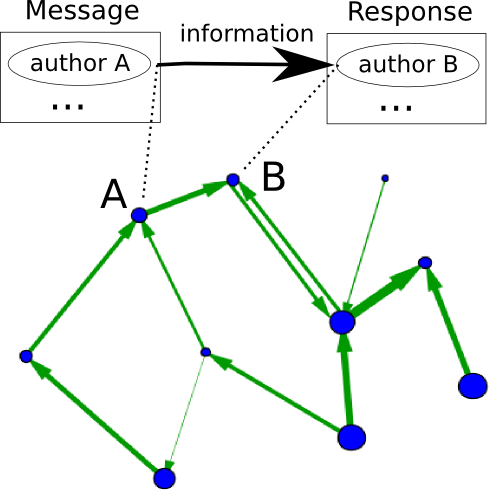
\includegraphics[width=0.5\textwidth]{figs/criaRede_}
    \caption{Formation of interaction network from email messages. Each vertex represents a participant. A reply message from participant B to a message from participant A is regarded as evidence that B received information from A. Multiple messages add ``weight'' to a directed edge. Further details are given in Section~\ref{intNet}.}
    \label{formationNetwork}
\end{figure}


Edges can be created from all antecedent messages on the message-response thread. We only linked the immediate antecedent to the new message's author, both for simplicity and for the valid objection that in adding two edges, $x\rightarrow y$ and $y\rightarrow z$, there is also a weaker connection between $x$ and $z$. Potential interpretations for this weaker connection are: double length, half weight or with one more ``obstacles''. This suggests pertinence of centrality measures that account for the connectivity with all nodes, such as betweenness centrality and accessibility~\cite{luMeasures,access}.


        \subsubsection{Sectioning networks in periphery, intermediary and hubs sectors}\label{sectioning}


Social networks tend to have a scale-free distribution of connectivity, and the primitive sectors (periphery, intermediary and hubs) can be derived from comparison with an Erd\"os-R\'enyi  network with the same number of edges and vertices~\cite{3setores}, as depicted in Figure~\ref{fig:setores}.
The degree distribution $\widetilde{P}(k)$ of an ideal
scale-free network $\mathcal{N}_f$ with $N$ vertices and $z$ edges has less
average degree nodes than the distribution $P(k)$ of an Erd\"os-R\'enyi
network with the same number of vertices and edges. Indeed, we define in this work the intermediary sector of a network to be the set of all the nodes whose degree is less abundant in the real network than on the Erd\"os-R\'enyi model:

\begin{equation}\label{criterio}
    \widetilde{P}(k)<P(k) \Rightarrow \text{k is intermediary degree}
\end{equation}

If $\mathcal{N}_f$ is directed and has no self-loops, the probability
of an edge between two arbitrary vertices is $p_e=\frac{z}{N(N-1)}$ (see Appendix~\ref{ap:ded}).
A vertex in the ideal Erd\"os-R\'enyi digraph with the same number of vertices and edges, and thus the same probability $p_e$ for the presence of an edge, will have degree $k$ with probability:

\begin{equation}
    P(k)=\binom{2(N-1)}{k}p_e^k(1-p_e)^{2(N-1)-k}
\end{equation}

The lower degree fat tail represents the border vertices, i.e. the peripheral sector or periphery where $\widetilde{P}(k)>P(k)$ and $k$ is lower and any intermediary sector value of $k$. The higher degree fat tail is the hub sector, i.e. $\widetilde{P}(k)>P(k)$ and $k$ is higher than any intermediary sector value of $k$. The reasoning for this classification is: 1) vertices so connected that they are virtually inexistent in networks connected at pure chance (e.g. without preferential attachment) are correctly associated to the hubs sector. Vertices with very few connections, which are way more abundant than expected by pure chance, are assigned to the periphery. Vertices with degree values predicted as the most abundant if connections are created by pure chance, near the average, and less frequent in scale-free phenomena, are classified as intermediary. 
\begin{figure}[!h]
    \centering
    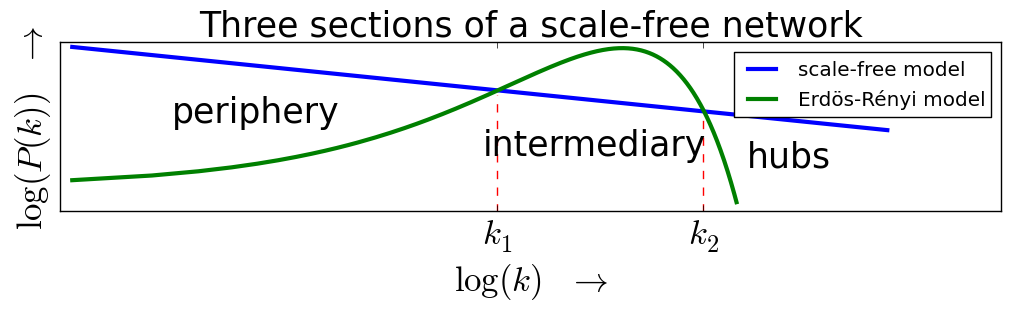
\includegraphics[width=0.5\textwidth]{figs/fser_}
    \caption{Degree distribution on scale-free and Erd\"os-R\'enyi ideal networks. The latter has more
        intermediary vertices, while the former has more peripheral and hub vertices. Sector borders are
        given by the two intersections $k_1$ and $k_2$ of the connectivity distributions. Characteristic degrees
    are in compact intervals of degree: $[0,k_1]$, $(k_1,k_2]$, $(k_2,k_{max}]$ for the three sectors considered (periphery, intermediary and hubs).}
    \label{fig:setores}
\end{figure}

To ensure statistical validity, bins can be chosen to contain at least $\eta$ vertices. Thus, each bin, starting at degree $k_i$, spans $\Delta_i=[k_{i},k_{j}]$ degree values, where $j$ is the smallest integer with which there are at least $\eta$ vertices with degree larger than or equal $k_i$, and less than or equal $k_{j}$. This changes equation~\ref{criterio} to:

\begin{equation}\label{criterio2}
    \sum_{x=k_i}^{k_j} \widetilde{P}(x) < \sum_{x=k_i}^{k_j} P(x) \Rightarrow \text{i is intermediary}
\end{equation}

If strength $s$ is used for comparison, $P$ remains the same, but $P(\kappa_i)$ with $\kappa_i=\frac{s_i}{\overline{w}}$ should be used for comparison, with $\overline{w}=2\frac{z}{\sum_is_i}$ the average weight of an edge and $s_i$ the strength of vertex $i$. For in and out degrees and strengths, comparison should be made with $\kappa_i=2k_i^{in}$, $\kappa_i=2k_i^{out}$, $\kappa_i=2\frac{s_i^{in}}{\overline{w}}$ and $\kappa_i=2\frac{s_i^{out}}{\overline{w}}$. Results of these criteria for network segmentation are discussed in Section~\ref{subsec:pih} and exhibited in Figures~\ref{fig:cpp10000} to~\ref{fig:lad50_} of Appendix~\ref{figures}.

Since different metrics can be used in the segmentation to identify the three types of vertices, various criteria can be defined, e.g. with a very stringent criterion according to which a vertex will only be classified as hub if it is so for all the metrics. After a careful inspection of possible combinations, these were reduced to six:

\begin{itemize}
\item Exclusivist criterion:  vertices are only classified if the class is the same according to all metrics. In this case, vertices classified (usually) does not reach 100\%, which is indicated by a black line in the figures of Appendix~\ref{figures}.
        \item Inclusivist criterion: a vertex has the class given by any of the metrics. Therefore, a vertex can belong to more than one class, and the percentages of members may add to more than 100\%, which is indicated by a black line in the figures of Appendix~\ref{figures}.
    \item Exclusivist cascade: vertices are only classified as hubs if they are hubs according to all metrics. Intermediary are the vertices classified either as intermediary or hubs with respect to all metrics. The remaining vertices are regarded as peripheral.
    \item Inclusivist cascade: vertices are hubs if they are so classified according to any of the metrics. The remaining vertices are classified as intermediary, if they belong to this category for any of the metrics. Peripheral vertices will then be those which were not classified as hub or intermediary with any of the metrics. 
    \item Exclusivist externals: vertices are only hubs if they are classified as such according to all the metrics. The remaining vertices are classified as peripheral if they fall into the periphery or hub classes by any metric. The rest of the nodes are classified as intermediary.
    \item Inclusivist externals: hubs are vertices classified as hubs according to any metric. The remaining vertices will be peripheral if they are classified as such according to any metric. The rest of the vertices will be intermediary vertices.
\end{itemize}



These compound criteria, and the simplification of possibilities listed above (exclusivist/inclusivist, criterion/cascade/externals) , can be formalized in strict mathematical terms, but this was considered out of the scope of the present article. Important here is to notice that the compound criteria can be used to examine network sections in the case of a low number of messages, such as in the last figures of Appendix~\ref{figures}.

Results from applying this classification method, i.e. the achievement of well defined sectors by comparison of the real network with the Erd\"os R\'enyi model, are reported in Section~\ref{subsec:pih} and Appendix~\ref{figures}.


\subsubsection{Topological measurements}\label{measures}

The topology of the networks was characterized with a small selection of the most standard measurements for each vertex, as follows:

\begin{itemize}
    \item Degree $k_i$: number edges linked to vertex $i$.
    \item In-degree $k_i^{in}$: number of edges ending at vertex $i$.
    \item Out-degree $k_i^{out}$: number of edges departing from vertex $i$.
    \item Strength $s$: sum of weights of all edges linked to vertex $i$.
    \item In-strength $s_i^{in}$: sum of weights of all edges ending at vertex $i$.
    \item Out-strength $s_i^{out}$: sum of weights of all edges departing from vertex $i$.
    \item Clustering coefficient $cc_i$: fraction of pairs of neighbors of $i$ that are linked.  The standard clustering coefficient for undirected graphs was used.
  \item Betweenness centrality $bt_i$: fraction of geodesics that contain the vertex $i$. Betweenness centrality index considered directions and weight, as specified in~\cite{faster}.
\end{itemize}

In order to capture symmetries in the activity of participants, the following metrics were introduced for a vertex $i$ (see Section~\ref{prevalence}):

\begin{itemize}
    \item Asymmetry: $asy_i=\frac{d_i^{in}-d_i^{out}}{d_i}$.
    \item Mean of asymmetry of edges: $\mu_i^{asy}=\frac{\sum_{j\in J_i} e_{ji}-e_{ij}}{|J_i|}$. Where $e_{xy}$ is 1 if there is and edge from $x$ to $y$, $0$ otherwise. $|J_i|$ is the number of neighbors of vertex $i$.
    \item Standard deviation of asymmetry of edges: $\sigma_i^{asy}=\sqrt{\frac{\sum_{j\in J_i}[\mu_{asy} -(e_{ji}-e_{ij}) ]^2  }{|J_i|}  }$
    \item Disequilibrium: $dis_i=\frac{s_i^{in}-s_i^{out}}{s_i}$.
    \item Mean of disequilibrium of edges: $\mu_i^{dis}=\frac{\sum_{j \in J_i}\frac{w_{ji}-w_{ij}}{s_i}}{|J_i|}$, where $w_{xy}$ is the weight of edge $x\rightarrow y$ and zero if there is no such edge.
    \item Standard deviation of disequilibrium of edges: $\sigma_i^{dis}=\sqrt{\frac{\sum_{j\in J_i}[\mu_{dis}-\frac{(w_{ji}-w_{ij})}{s_i}]^2}{|J_i|}}$
\end{itemize}

   \subsection{Evolution of the networks}
The evolution of the networks was observed within a fixed number of messages, the window size $ws$, that shifts in the message timeline.
The $ws$ used were 50, 100, 200, 400, 500, 800, 1000, 2000, 2500, 5000 and 10000. Within a same $ws$, the number of vertices and edges vary in time, as do other network characteristics. 

        \subsection{Visualization of network evolution}
The evolution of the networks was visualized with animations, image galleries and online gadgets made for this research~\cite{animacoes,galGMANE,appGMANE}. Such visualizations were crucial to guide research into the most important features of network evolution, and prompted us to capture the prominence of topological metrics along time using mean and standard deviations (see Section~\ref{measures} and Appendix~\ref{sec:pcat}), in addition to the size of the three sectors in a timeline fashion (Appendix~\ref{figures}). Visualization of network structure was specially useful as part of the email lists data mining, from which parts of relevant structures and results were driven. See Appendix~\ref{sec:fure} for further directions about visualization and text mining concerning the results herein presented, with dedicated articles.


    \subsection{Typological deepening}\label{subsec:typ}
There are other ways to split and characterize networks. To point a common example, the center of the network is defined as all the nodes whose maximum distance to any other node is the radius (the radius is the minimum maximum distance to all vertices , i.e. the radius is the minimum eccentricity). 
In the same framework, the periphery (as opposed to the center) consists of the nodes whose maximum distance to any node is the diameter (diameter being the maximum geodesic on the network). Accordingly, the intermediary sector can be defined as the nodes that are not in the center or in the periphery. Interestingly, in the email networks analyzed, with such criteria, the center can often be a factor of 4 times larger than the periphery and the intermediary group often exceeds 90\% of the nodes~\cite{networkx}.

Models of human dynamics can be used to predict and classify activity. In this case, agent activity is commonly considered a Poisson process, as a consequence of the randomly distributed events in time. Even so, evidence-based models suggests that human activity patterns follow non-Poisson statistics, characterized by a long tail of inactivity with bursts of rapidly occurring events~\cite{barabasiHumanDyn,barabasiPhone}. Emails are reported as having a heavy tailed distribution with $\alpha=1$, together with web browsing and library loans~\cite{barabasiHumanDyn}.

Typologies can also be conveniently adapted from psychiatric, psychological and psychoanalytic theories.
Concerning empirical research,
Theodor Adorno is a core conceiver of an one-of-a-kind typology that resulted from observing authoritarian
personality traces to detect Nazism adoption, antisemitism and potential fascists, depicted as an authoritarian syndrome~\cite{adorno}.

%Influenced by Social and Psychoanalytic Theories, Adorno et all applied a %questionnaire to individuals, from which they reached a position in the the %``F Scale'', to verify etnocentric, conservatory and antidemocratic %trends~\cite{adorno}. From psychoanalitic interviews and the F Scale, they %derived a typology, which gathers prejudice-inclined traces in personality. %Both, low and high scores are considered with prejudicial traces. This %typology has nine authoritarian types, the six types with high score in the F %Scale: surface resentment, conventional, authoritarian, rebel and psychopath, %crank, manipulative; and three of the five types with low score in the F %Scale: rigid, protesting, impulsive, easygoing, genuine liberal. Each side of %the dipole has a rank of intensity that increases as the order written above.


Other classic typologies of interest include Jung's extroversion-introversion trait with four modes of orientation. This four modes are divided in two perceiving functions (sensation and intuition) and two judging functions (thinking and feeling), each individual manifesting one of these four modes as dominant, and each mode expressed primarily as introverted or extroverted~\cite{jung}. Myers-Briggs Type Indicator extrapolated Jungian theories into a questionnaire and added perceiving and judging as a fourth dipole~\cite{myers}. Even plain Freudian criteria, such as neurosis, psychosis, perversity and denegation, can be used directly for such categorization, as they have verbal and behavioral typical traces~\cite{freud,freud2}.

It was considered central to benefit from key human typologies, both by describing types and by further characterizing classes in the terms encountered. A primitive physics-based typology is described in Section~\ref{sec:pty} as a consequence of the periphery, intermediary and hub sectors yielded by comparing the real networks with the Erd\"os R\'enyi model.
Also, ethic and moral issues are developed by such legacy. For example, Adorno et al. conceptualized that personality is dynamic, not static or immutable, and that recognizing this was important for an ethic empirical study of human authoritarian traces~\cite{adorno}.
Indeed, this dynamic typological approach is so vital to secure an ethic study of human systems that our epigraph is devoted to make this point explicit.

%    \subsection{Other analisys of interest}
%
%        \subsubsection{Textual content}
%        \subsubsection{Geographical localization}

\section{Results and discussion}

\subsection{Constancy and discrepancy of activity along time}\label{constDisc}
One remarkable feature from the analysis is that the activity along time is practically the same for all lists.

\subsubsection{Seconds and minutes}
The incidence of messages at each second of a minute and at each minute of an hour is compatible with uniform distribution simulations\footnote{Numpy version 1.6.1, ``random.randint'' function, was used for simulations.}. Messages were slightly more evenly distributed in all lists: for both seconds and minutes  $\frac{max(incidence)}{min(incidence)} \in (1.26,1.275]$. Simulations reach these values  but have in average more discrepant higher and lower peaks $\xi=\frac{max(incidence')}{min(incidence')} \Rightarrow \mu_\xi=1.2918 \text{ and } \sigma_\xi=0.04619$.

\subsubsection{Hours of the day}
Higher activity was observed between noon and 6pm, followed by the time period between 6pm and midnight. Around 2/3 of the whole activity takes place from noon to midnight, as can be seen in Table~\ref{dia}. Nevertheless, the activity peak occurs around midday, with a slight skew toward one hour before noon.

\subsubsection{Days of the week}
Higher activity was observed during weekdays, specially for the CPP and MET lists (see Table~\ref{semana}). The decrease of activity on weekends reaches at least one third, and two thirds in extreme cases.

\subsubsection{Days along the month}
Table~\ref{mes} shows activity along the month. Variation of activity in the days along the month is less prominent, one cannot point much more than a - probably not statistically relevant - tendency of first and second weeks to be more active. The most important trait seems to be homogeneity. Last days of the month (29, 30 and 31) are not present in every month, and observed activity is proportional to incidence rates.

\subsubsection{Months and larger divisions of the year}
 Activity is concentrated in Jun-Aug for MET and LAD, and in Dec-Mar for CPP, LAU and LAD (see Table~\ref{ano}). These observations fit academic calendars, vacations and end-of-year holidays.

\subsection{Scalable fat-tail structure}\label{subsec:pih}
There is a concentration of hub activity and of vertex with few connections. Table~\ref{autores} is dedicated to exposing this well known and expected distribution of activity among participants.

The distribution of vertices in the three sectors defined in Section~\ref{sectioning} (hubs, intermediary, periphery) is remarkably stable along time, provided that a sufficiently large sample of 200 or more messages is considered. Moreover, the same distribution applies to the networks of all the four email lists, to which are dedicated the various figures in Appendix~\ref{figures}. If, for instance, strength is taken as the criterion to define the sectors, $\approx 5\%$ of the vertices are found to be hubs, $\approx [15-20]\%$ are intermediary and $\approx [75-80]\%$ are peripheral, which is consistent with the literature~\cite{secFree}. If the degree is used for classification, hubs can reach $10\%$ of all vertices, i.e. classification with strength yields half the number of hubs as plain degree. These results hold for in and out degrees and strengths. Stable distributions can also be obtained for 200 of less messages if classification of the three sectors is performed with one of the compound criteria established in Section~\ref{sectioning}. In fact, a minimum window size for observation of more general properties can be inferred by monitoring the giant component and the degeneration of the hub, intermediary and peripheral sections. This degeneration is critical in the span of 50-100 messages. Even so, using a compound criterion, such as exclusive cascade of Figure~\ref{fig:cpp250_}, the networks seem to hold their basic structure with as few as 20-50 messages. This indicates that concentration of activity and the abundance of low-activity participants take place even with very few messages, which is highlighted in the last figures of Appendix~\ref{figures}.

For the histograms used in the classification process (see Section~\ref{sectioning}), the use of at least $\eta$ vertices for each bin did not yield significant differences.
That was understood as a consequence of the observation scale:
\emph{There are between 20 and 200 participants in the message window sizes used to derive most of the results ($ws \in [200,1500]$ messages). As peripheral vertices are abundant and span few degrees, there are more than $\eta$ vertices with each low degree value. For the case of higher degrees, one should consider that with the $ws$ used, each participant is $p \in [0.1\%,0.5\%]$ of all participants. Therefore, if incident connectivity is very improbable in an Erd\"os R\'enyi network (less than $p$, the probability that a single participant represents when the histogram is normalized to the density function), than it is not an intermediary connectivity, but a hub. Therefore, using at least $\eta$ vertices for each bin did not impact the results.}

    \subsection{Prevalence of centrality over symmetry and symmetry over clusterization}\label{prevalence}
The principal component (PCA~\cite{pca}) exhibited a ponderation of centrality measures: degrees, strengths and betweenness centrality. Clustering coefficient is presented in almost perfect orthogonality.
Symmetry of edges have been reported as bonded to different roles played by participants and relations~\cite{newmanEvolving}, and dispersion was more prevalent in symmetry related measures than clustering coefficient.
This composition of the principal component suggests that all six degree and strength measures are equally important for system characterization, although it is known that they do not relate to the same participation characteristics.
The contribution from the distinct metrics to network topology variance is very similar for all the networks considered, and did not vary with time. This stability in network behavior is remarkable, as shown by the very small standard deviations of the contributions from the metrics along time in Appendix~\ref{sec:pcat}.

The dispersion is mostly presented by degree, strength and betweenness centrality, as indicated in Tables~\ref{compPCA0} and~\ref{compPCA} for the LAU list (similar results are obtained for the other lists and omitted here for simplicity). The standard deviations are small, which means that the first and second components varies little with time.
 Degree and strength are highly correlated, with Spearman correlation coefficient $\in [0.95,1]$ and Pearson coefficient $\in [0.85,1)$ for $ws>1000$. The corresponding PCA plot for the two first components is shown in Figure~\ref{PCA}, where each vertex is colored according to the sector they belong. As expected, peripheral vertices have very low values in the first component and greater dispersion in the second component. 
The plot of clustering coefficient versus degree in Figure~\ref{clust} is similar to the PCA in Figure~\ref{PCA}.

The PCA plot in Figure~\ref{PCA2}, where all metrics are considered, reflects symmetry-related relevance for the variance. This is shown in Table~\ref{compPCA2}  where the clustering coefficient is only relevant for the third principal component (with contributions from out-degree and out-strength). It is concluded that the symmetry-related measurements can be more meaningful in characterizing interaction networks (and their participants) than the clustering coefficient, especially for hubs and intermediary vertices, which are more dispersed in Figure~\ref{PCA2} than in Figure~\ref{PCA}. 


\begin{figure} 
   \centering
        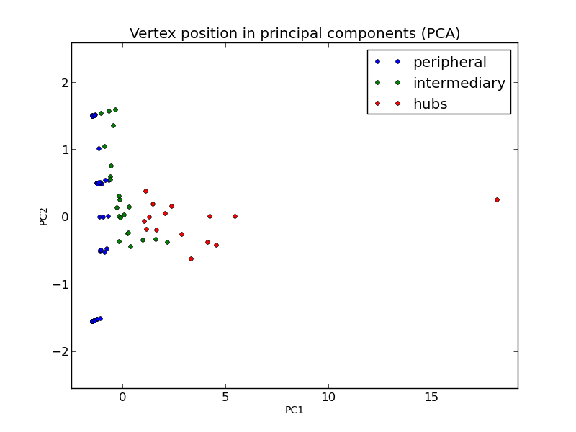
\includegraphics[width=\columnwidth]{figs/ev0pr3PCA}
    \caption{Scatter plot of vertices for the LAU list using two principal components from a PCA in the metrics space of in- and out- degree and strength, betweenness centrality and clustering coefficient, as specified in Section~\ref{measures}. Principal component is a weighted average of centrality measures: degrees, strengths and betweenness centrality. Second component is mostly clustering coefficient. Table~\ref{compPCA} shows the composition of principal components.  Similar plots were obtained for all window sizes  $ws\;\in\;[500,10000]$, and for the networks of the other email lists, which exposes a common relation held by degree, strength and betweenness measures to clustering coefficient.}
    \label{PCA}
\end{figure}



\begin{figure} 
   \centering
        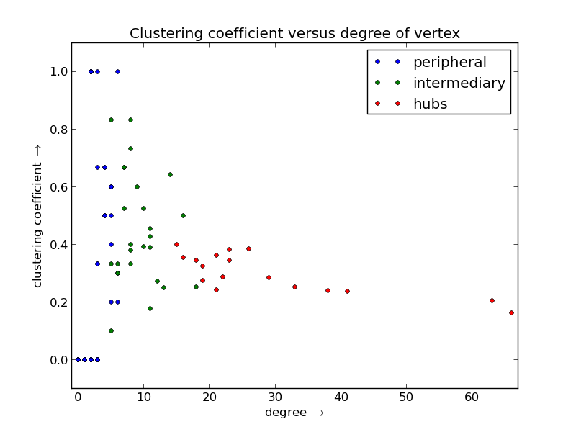
\includegraphics[width=\columnwidth]{figs/ev0pr11CC}
    \caption{Clustering coefficient versus degree of vertices with a window size of $ws = 1000$ email messages, LAU list. The general layout is consistent with the literature: most connected vertices have low clusterization while higher clusterization is gradually more incident as the number of connections is lowered.}
    \label{clust}
\end{figure}

\begin{figure} 
   \centering
        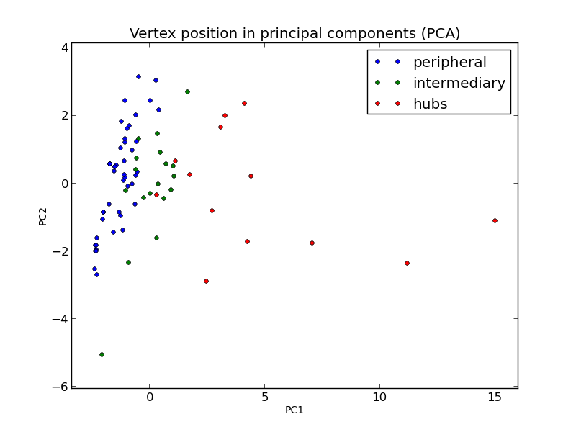
\includegraphics[width=\columnwidth]{figs/ev0pr1PCA}
    \caption{Scatter plot of vertices for the LAU list using two principal components from a PCA in the metrics space of (in-,  out- and total) degree, (in-,  out- and total) strength, betweenness centrality, clustering coefficient and symmetry-related measurements. The composition of the first three components are shown in Table~\ref{compPCA2} and measure details in Section~\ref{measures}. Most importantly, clustering coefficient is only relevant for third component, being second component representative of symmetry measurements of vertex interactions. Dispersion suggests symmetry related measures are more powerful for characterizing interaction networks than clustering coefficient, specially for hubs and intermediary vertices.}
    \label{PCA2}
\end{figure}

    \subsection{Primitive typology: the activity of participants from different sectors}\label{sec:pty}

This work is aimed at finding common characteristics among (email) interaction networks. Analysis involved primary measures observance and a formal criteria for coherent ratios of hub, intermediary and hub sectors. In this process, inspection done by visualizations and raw data manipulations suggests agents typological peculiarities. These are initial observations, which inspired this article and other ongoing research:

\begin{itemize}
    \item Core hubs usually have intermittent activity. Very stable activity was found on MET hubs, which motivated its integration to this work. There are reports in the literature of greater stability of participation in smaller communities~\cite{barabasiEvo}, which is the reason why the smaller number of participants in MET was considered coherent with the stable activity of hubs.
    \item Typically, the activity of hubs is trivial: they interact as much as possible, in every occasion with everyone. The activity of peripheral vertices also follows a simple pattern: they interact very rarely, in very few occasions. Thereafter, intermediary vertices seem responsible for the network structure. For example, intermediary vertices may exhibit preferential communication to peripheral, intermediary, or hub vertices; can be marked by stable communication partners; can involve stable or intermittent patterns of activity.
    \item Some of the most active participants receive many responses with relative few messages sent, and rarely are top hubs. These seem as authorities and contrast with participants that respond much more than receive responses.
    \item The most obvious community structure, as observed by high clustering coefficient, is found only in peripheral and intermediary sectors.
\end{itemize}


This ``primitive typology'', characterized by peripheral, intermediary and hub types, can be further scrutinized using concepts involved in other typologies, such Meyer-Briggs, Pavlov or F-Scale. This has no pretension of being a direct result of numeric analysis, it is a description refinement of the found structure, in typological terms, and coherent with complex networks literature. Although initial, this bridges human and exact sciences in the most pertinent way authors were able to, as is herein considered a result.

Another typology suggested by results is about the networks themselves. In accordance with previous research results~\cite{barabasiEvo}, this and paired articles~\cite{rcText,versinus} reports a dipole in human interaction network types: networks with few and stable agents, and (relative) many threads per amount of messages contrasts with networks with many agents of intermittent activity and (relative) few threads per amount of messages.
 
\section{Conclusions}
The characterization of interaction networks resulted from stability observations. Along temporal activity statistics, this work reports the stability of the principal components (in the concentration of dispersion and composition) and of the ternary partitioning (periphery, intermediary, hubs) relative sizes, evident in the comparison with the Erd\"os-R\'enyi model. These results suggested typologies for both agents and the networks.


    \subsection{Further work}
The task of delivering a first and general characterization of chosen interaction networks involved a larger effort. The different aspects covered requires not only different analytical background, but also considerations about textual production and social psychology. These are receiving attention within dedicated works and are summarized in this section.

        \subsubsection{Constancy of general characteristics eases tipologization}

Regarding topological aspects of interaction networks, further work should inspect other measures in each of the three connective sectors: hubs, intermediary and periphery.

Observance of attributes with greater contribution to principal components of LDA should reveal best chances to present these three sections as clusters in the network measurements space. Another possibility, specially for a brute-force characterization of such sectors, is to remove vertices with degree close to $k_1$ or $k_2$ depicted in figure~\ref{fig:setores}. The subtraction $\widetilde{P}(k)-P(k)$ (see Section~\ref{subsec:typ}) results in two positive clusters for periphery and hubs, and a negative cluster for intermediary vertices. This might support classification of the three sectors by clustering, a more traditional approach to classification.

Observed networks were coherent with literature in different aspects, such as concentration of activity, and clusterization versus connectivity patterns. Even so, analysis of data from other virtual environments, such as Facebook, Twitter and LinkedIn, might help understanding how general are these structures and what are convenient uses.

A paired article  is dedicated to textual production of the network sectors~\cite{rcText}. Resulting knowledge purposes networks and participants typologies, and both topological and textual analysis should foster characterization of interaction networks and participation incidences.
Stability reported in this article eases tipologization of outliers and more usual participation patterns. See Appendix~\ref{sec:fure} for further consideration of works related to presented results.

        \subsubsection{Results exploitation}
On the technological trend, usage of such characteristics are taking place in linked data and electronic government technologies~\cite{ops,opa,ensaio}. Further steps involve elaboration and tests of social dynamics that takes advantages of these results. These results are also being used for anthropological physics experiments~\cite{anPhy} and knowledge acquisition~\cite{rcText}.

\begin{acknowledgments}
Renato Fabbri is grateful to CNPq (process: 140860/2013-4,
project 870336/1997-5), United Nations Development Program (PNUD/ONU, contract: 2013/000566; project BRA/12/018)  and 
the Postgraduate Committee of the IFSC/USP. This author is also grateful for
the American Jewish Committee for maintaining an online copy of the Adorno book
used on the epigraph~\cite{adorno}. Authors thank GMANE creators and maintainers, specifically: GMANE is run by Lars Magne Ingebrigtsen, and the administrators are Tom Koelman, Jason R. Mastaler, Steinar Bang, Jon Ericson, Wolfgang Schnerring, Sebastian D.B. Krause, Nicolas Bareil, Raymond Scholz, and Adam Sjøgren. Authors thank referred email lists communities and welcome feedback as core contribution to this, and similar, research.
\end{acknowledgments}


%%%%%%%%%%%%%%%%%%%%%%%%%%%%%%%%%%%%%%%
\appendix
\section{Edge existence probability in a directed network without self-loops}\label{ap:ded}
Be $\mathcal{N}$ a directed network without self-loops with $z$ edges and $N$ vertices. The probability that an edge exists between two arbitrary vertex is $p_e=\frac{z}{max( \text{number of edges} |\ \text{N vertices})}$, where $max( \text{number of edges} |\ \text{N vertices})=2[(N-1)+(N-2)+...+1]=2[\sum_1^{N-1}i]=2[\frac{N(N-1)}{2}]$ is the maximum number of edges for a network with $N$ vertices. Therefore:
\begin{align}
    p_e&=\frac{z}{max( \text{number of edges} |\ \text{N vertices})} \nonumber \\
       &=\frac{z}{2[(N-1)+(N-2)+...+1]}=\frac{z}{2\frac{N(N-1)}{2}} \nonumber \\
   p_e &=\frac{z}{N(N-1)}
\end{align}

\section{Work related to the results}\label{sec:fure}
Unreciprocated edges often exceed 50\%, which matches empirical evidence~\cite{newmanEvolving}. Although no correlation of topological characteristics and geographical position was found in a pertinent study~\cite{barabasiGeo}, geographical incidences should be present in further refinement of the analysis.

The seminal Nature Letter by Palla, Barab{\'a}si and Vicsek~\cite{barabasiEvo} has strong confluence with this work, suggesting that smaller size of MET community is responsible for the stronger hubs observed.

Controllability of these networks is also an uncovered issue. These has unintuitive properties and might bring into forefront crucial differences between email interaction networks and interaction networks in Facebook or Twitter~\cite{barabasiControlCapacity,barabasiControlCentrality,barabasiControllability}.

Gender related behavior in mobile phone datasets has been reported~\cite{barabasiSex} and can be further investigated in non-private email lists with hundreds or thousands of participants~\cite{GMANE}.

\subsection{Paired article to analyse textual production}
Significant differences in the textual production of each connective sector of the network (periphery, intermediary, hubs) is reported in an article by the same research group~\cite{rcText}. Most importantly, linguistic differences are more prominent between the sectors of a same network than between the same sector in different lists. 

\subsection{The Versinus visualization method for evolving complex networks}
To visualize network evolution, the Versinus method was developed. The method is simple and consists in the placement of each vertex along a sinusoid and a line. In the resulting fixed layout, the time evolution takes place.  Even so, fellow researchers repeatedly asked for an article describing Versinus, and it was written in 2013~\cite{versinus}.

\subsection{Typology of online agents}
A core purpose of the present article, dedicated to stability in interaction networks, and the article about textual production~\cite{rcText} is to derive a sound typology of online agents, with quantitative criteria driven from physics (to the extent possible). This is a work under construction, with preliminary elaborations in Section~\ref{sec:pty}, but should be published in near future.


\section{Data and scripts}\label{scripts}
Messages are downloaded from the GMANE database by RSS in the mbox email text format. 
They are requested one by one to avoid reaching maximum size of the requests accepted by
GMANE API.

Every message has about 30 fields, from which the following are crucial
for the present work:
\begin{itemize}
    \item ``From'' field, as it specifies the sender of the message, in the usual format of ``First\_name Last\_Name $<email>$''.
    \item ``Date'' field, which is given with the resolution of a second.
    \item ``Message-ID'', important to state antecedent/consequent relation between messages and therefore from an author to a replier.
    \item ``References'', has the ID of the message it is an answer to, if any, and earlier messages in the thread.
\end{itemize}

Field ``In-Reply-To'' has only the ID of the message it replies and can be sometimes
a shortcut or an alternative to ``References''. Also, the textual content of the messages,
accessed through ``payload'' method of the mbox message object, is of central interest and
the authors dedicated an article to include the textual content of the messages to the analysis~\cite{rcText}.

\subsection{Python scripts}\label{ap:os}
Basic constructs for obtaining all results are the product of scripts written in the Python programming language. These are kept in a public git repository for backup and sharing with research community~\cite{scriptsFim}. Core scripts, for deriving structures and results exhibited in this article, are in the LEIAME file.


\subsection{Third party libraries and software}
The programming framework used 
is mainly Python-based, with emphasis on usual
scientific tools. More specifically,
scripts where written for 2.7.3 version of Python,
with the following third party libraries: Numpy, Pylab/Matplotlib, NetworkX, IGraph.
Behind the scenes, Graphviz is accessed via PyGraphviz to make network drawings.
\section{Tables}\label{sectables}
\clearpage
\subsection{PCA tables}\label{sec:pcat}

\begin{table}[H]
  \centering
  \caption{Principal components composition in the simplest case: with degree, clustering coefficient and betweenness centrality. LAU list, $ws=1000$ messages in 20 disjoint positioning was used for statistics. The first component is a weighted average of degree and betweenness centrality. The second component is mostly clustering coefficient. The first and second components represent more than 95\% of total variance. The $\lambda$ bottom line holds the percentage of total variance attributed to each component.}
  \begin{tabular}{|l|c|c| c|c| c|c|}\hline
 & \multicolumn{2}{c|}{PC1}          & \multicolumn{2}{c|}{PC2} & \multicolumn{2}{c|}{PC3}  \\\hline
       & $\mu$            & $\sigma$ & $\mu$         & $\sigma$ & $\mu$ & $\sigma$  \\\hline
$d$       & {\bf 48.02}   & 1.39     & 2.82          & 1.74     & 48.09  & 0.32 \\
$cc$      & 4.12          & 2.94     & {\bf 90.45}   & 3.98     & 3.98  & 0.77 \\ 
$bt$      & {\bf 47.87}   & 1.55     & 6.74          & 4.08     & 47.93 & 0.46 \\ \hline
$\lambda$ & 64.67         & 0.52     & 33.26         & 0.23     & 2.08  & 0.40 \\ \hline
  \end{tabular}
  \label{compPCA0}
\end{table}





\begin{table}
  \centering
  \caption{Principal components composition in percentages. LAU list, $ws=1000$ messages in 20 disjoint positioning was used for statistics. First component is a weighted average of degree and strength and betweenness centrality. The second component is mostly related to the  clustering coefficient. The first and second components represent more than 90\% of the variance.}
  \begin{tabular}{|l|c|c| c|c| c|c|}\hline
 & \multicolumn{2}{c|}{PC1} & \multicolumn{2}{c|}{PC2} & \multicolumn{2}{c|}{PC3}  \\\hline
       & $\mu$ & $\sigma$ & $\mu$ & $\sigma$ & $\mu$ & $\sigma$  \\\hline
$d$       & {\bf 14.58} & 0.14 & 0.43  & 0.35 & 1.51  & 1.08 \\
$d^{in}$  & {\bf 14.12} & 0.14 & 1.71  & 1.22 & 17.80 & 6.20 \\
$d^{out}$ & {\bf 13.95} & 0.12 & 2.80  & 1.83 & 21.15 & 5.62 \\
$s$       & {\bf 14.48} & 0.13 & 0.78  & 0.65 & 5.51  & 4.71 \\ 
$s^{in}$  & {\bf 14.10} & 0.14 & 2.17  & 1.28 & 17.32 & 6.11 \\ 
$s^{out}$ & {\bf 14.05} & 0.13 & 2.08  & 1.14 & 19.31 & 4.86 \\ \hline
$cc$      & 0.99        & 0.70 & {\bf 83.38} & 4.83 & 2.75  & 1.62 \\ 
$bt$      & {\bf 13.73} & 0.19 & 6.65  & 1.31 & 14.66 & 10.14 \\ \hline
$\lambda$ & 81.80 & 0.83 & 12.53 & 0.09  & 3.24 & 0.62 \\ \hline
  \end{tabular}
  \label{compPCA}
\end{table}


\begin{table}
  \centering
  \caption{Principal components formation with symmetry-related metrics (see Section~\ref{measures}). LAU list, $ws=1000$ messages in 20 disjoint positioning was used for statistics. In this case, clusterization is pushed to the third principal component. The second component is primarily derived from symmetry measurements, but also out-degree and out-strength, and disequilibrium standard deviation. Betweenness centrality again has a role similar to degree, but weaker. The clusterization component combines with disequilibrium, while asymmetry is combined to out-degree and out-strength. The three components have in average 80.36\% of the variance.}
  \begin{tabular}{|l|c|c| c|c| c|c|}\hline
 & \multicolumn{2}{c|}{PC1} & \multicolumn{2}{c|}{PC2} & \multicolumn{2}{c|}{PC3}  \\\hline
       & $\mu$ & $\sigma$ & $\mu$ & $\sigma$ & $\mu$ & $\sigma$  \\\hline
$d$            & {\bf 11.51} & 0.42 & 2.00  & 0.76 & 2.39  & 0.49 \\ 
$d^{in}$       & {\bf 11.45} & 0.34 & 2.86  & 0.91 & 1.68  & 0.67 \\
$d^{out}$      & {\bf 10.68} & 0.60 & {\bf 7.43}  & 1.00 & 3.00  & 1.02 \\
$s$            & {\bf 11.37} & 0.42 & 1.75  & 0.71 & 4.31  & 0.63 \\ 
$s^{in}$       & {\bf 11.33} & 0.35 & 2.39  & 1.10 & 3.69  & 0.86 \\ 
$s^{out}$      & {\bf 10.74} & 0.55 & {\bf 6.14}  & 1.05 & 4.75  & 0.98 \\ \hline
$cc$           & 0.91        & 0.64 & 2.68  & 1.67 & {\bf 22.27} & 6.43 \\ 
$bt$           & {\bf 10.87} & 0.38 & 1.17  & 0.93 & 4.03  & 1.42 \\ \hline
$asy$          & 3.99        & 1.45 & {\bf 18.13} & 1.67 & 2.55  & 1.77 \\
$\mu_{asy}$    & 4.15        & 1.40 & {\bf 17.07} & 1.78 & 2.49  & 1.67 \\
$\sigma_{asy}$ & 1.21        & 0.67 & {\bf 17.49} & 0.79 & 3.29  & 2.33 \\
$dis$          & 5.78        & 0.51 & 1.94  & 1.28 & {\bf 24.75} & 3.73 \\
$\mu_{dis}$    & 0.79        & 0.49 & {\bf 14.00} & 1.14 & 3.73  & 3.13 \\
$\sigma_{dis}$ & 5.18        & 0.72 & 4.93  & 2.48 & {\bf 17.04} & 4.78 \\ \hline
$\lambda$      & 51.09       & 1.07 & 20.04 & 1.31 & 9.23  & 6.63 \\ \hline
  \end{tabular}
  \label{compPCA2}
\end{table}

\clearpage

\subsection{Tables for activity along time and among participants}\label{tabTime}

\begin{table}
    \caption{Distribution of activity among agents. First column is dedicated to percentage of messages sent by the most active participant. Column for the first quartile ($1Q$) exhibits minimum percentage of participants responsible for at least 25\% of total messages. Similarly, the column for the first three quartiles $1-3Q$ exhibits minimum percentage of participants responsible for 75\% of total messages. The last decile $10D$ column has maximum percentage of participants responsible for 10\% of messages.}
\begin{center}
    \begin{tabular}{ | l ||  c | c | c | c | }
        \hline
        list & hub & $ 1Q $ & $ 1-3Q $ & $10D$ \\ \hline
    CPP & 14.41 & 0.19 (27.8\%) & 4.09 (75.13\%) & 83.65 (-10.04\%)   \\ 
    MET & 11.14 & 0.81 (30.61\%) & 8.33 (75,11\%) & 80.49 (-10.02\%)  \\ 
    LAU & 2.78 & 1.10 (25.16\%) & 13.02 (75,04\%) & 67.37 (-10.03\%) \\ 
    LAD & 4.00 & 0.95 (25.50\%) & 11.83 (75,07\%) & 71.13 (-10.03\%) \\\hline
    \end{tabular}
\end{center}
\label{autores}
\end{table}


\begin{table*}
%\tiny
    \caption{Percentage of activity ($100\frac{\text{counted messages}}{\text{total messages}}$) in each hour, 6 hours and 12 hours. Maximum activity rates are in bold. In 1h columns, minimum activity is also bold. The less active period of the day is around 4-6h. Maximum activity is between 10-13h. Afternoon is most active in 6h division of the day. The noon has $\approx \frac{2}{3}$ of 24h activity. }\label{dia}
\begin{center}
    \begin{tabular}{ |l|| c|c|c| c|c|c| c|c|c| c|c|c|}
        \hline
    & \multicolumn{3}{c|}{CPP} & \multicolumn{3}{c|}{MET} & \multicolumn{3}{c|}{LAU} & \multicolumn{3}{c|}{LAD}  \\ \hline
    & 1h   & 6h & 12h &   1h & 6h & 12h &   1h & 6h & 12h &   1h & 6h & 12h \\ \hline\hline
0h  & 3.66 & \multirow{6}{*}{10.67} & \multirow{12}{*}{33.76} & 2.87  & \multirow{6}{*}{7.15} & \multirow{12}{*}{29.33} & 3.58 & \multirow{6}{*}{10.14} &  \multirow{12}{*}{36.88} & 4.00 & \multirow{6}{*}{10.77} & \multirow{12}{*}{33.13} \\
1h  & 2.76 &                        &                         & 1.77  & & &  2.22 & & & 2.52 & & \\
2h  & 1.79 &                        &                         & 1.04  & & & 1.63 & & & 1.79 & & \\
3h  & 1.10 &                        &                         & 0.64  & & & 1.06 & & & 1.06 & & \\
4h  & {\bf 0.68} &                        &                         & 0.47  & & &  0.84 & & & 0.75 & & \\
5h  & 0.69 &                        &                         & {\bf 0.38}  & & & {\bf 0.82} & & & {\bf 0.66} & & \\\cline{3-3}\cline{6-6}\cline{9-9}\cline{12-12}
6h  & 0.83 & \multirow{6}{*}{23.09} &                         & 0.72  & \multirow{6}{*}{22.18} & & 1.17 & \multirow{6}{*}{26.74} & & 0.85 & \multirow{6}{*}{22.36} &  \\
7h  & 1.24 &                        &                         & 1.33  & & & 2.37 & & & 1.56 & & \\
8h  & 2.28 &                        &                         & 2.67  & & & 3.54 & & & 2.96 & & \\
9h  & 4.52 &                        &                         & 4.40  & & & 6.04 & & & 4.68 & & \\
10h & 6.62 &                        &                         & 6.29  & & & {\bf 6.83} & & & 5.93 & & \\
11h & {\bf 7.61} &                        &                         & 6.78  & & & 6.79 & & & 6.40 & & \\\hline
12h & 6.44 & \multirow{6}{*}{\bf 37.63} & \multirow{12}{*}{\bf 66.24} & {\bf 7.33}  & \multirow{6}{*}{\bf 42.22} & \multirow{12}{*}{ \bf 70.66} & 6.11 & \multirow{6}{*}{\bf 35.65} &  \multirow{12}{*}{ \bf 63.12} & {\bf 6.41} & \multirow{6}{*}{\bf 37.25} &  \multirow{12}{*}{\bf 66.87} \\
13h & 6.04 &                        &                         & 7.08  & & & 6.26 & & & 6.12 & & \\
14h & 6.47 &                        &                         & 7.09  & & & 6.38 & & & 6.33 & & \\
15h & 6.10 &                        &                         & 7.14  & & & 5.93 & & & 5.98 & & \\
16h & 6.22 &                        &                         & 6.68  & & & 5.52 & & & 6.40 & & \\
17h & 6.36 &                        &                         & 6.89  & & & 5.46 & & & 6.02 & & \\\cline{3-3}\cline{6-6}\cline{9-9}\cline{12-12}


18h & 6.01 & \multirow{6}{*}{28.61} &                         & 5.99  & \multirow{6}{*}{28.44} & & 5.24 & \multirow{6}{*}{27.46} & & 5.99 & \multirow{6}{*}{29.63} & \\
19h & 5.02 &                        &                         & 5.23  & & & 4.52 & & & 5.03 & & \\
20h & 4.85 &                        &                         & 4.98  & & & 4.55 & & & 4.63 & & \\
21h & 4.38 &                        &                         & 4.37  & & & 4.42 & & & 4.59 & & \\
22h & 4.06 &                        &                         & 4.24  & & & 4.51 & & & 4.88 & & \\
23h & 4.30 &                        &                         & 3.64  & & & 4.23 & & & 4.53 & & \\\hline
    \end{tabular}
\end{center}
\end{table*}



\begin{table}[h]
    \caption{Percentage of activity on days along the week. Weekend days are at least $\frac{1}{3}$ less active and can reach $\frac{1}{3}$ of activity. MET concentrates activity in weekdays the most, leaving only 13.98\% of total activity to Saturday and Sunday. LAU is the one that less concentrates activity in weekdays, reaching 20.94\% of total activity in weekends. These might suggest professional relation of CPP and MET participants to the topics of interest, or a hobby relation of LAU and LAD participants.}
\begin{center}
    \begin{tabular}{ | l |  c | c | c | c | c |   c | c |}
        \hline
        & Mon & Tue & Wed & Thu & Fri & Sat & Sun  \\ \hline
        CPP & 17.06 & 17.43 & 17.61 & 17.13 & 16.30 & 6.81 & 7.67 \\ \hline
        MET & 17.53 & 17.54 & 16.43 & 17.06 & 17.46 & 7.92 & 6.06 \\ \hline
        LAU & 15.71 & 15.80 & 15.88 & 16.43 & 15.13 & 10.13 & 10.91 \\ \hline
        LAD & 14.91 & 17.73 & 17.01 & 15.40 & 14.25 & 10.39 & 10.30 \\\hline
    \end{tabular}
\end{center}
\label{semana}
\end{table}


\begin{table*}
%\tiny
    \caption{Activity along the days of the month. The pattern is to have no clear prevalent period. One might point a slight tendency for the first two weeks to be more active, although this table does not present statistical foundation for such an assumption. For the scope of this study, differences of activity along the month is assumed to be inexistent.}
\begin{center}
    \begin{tabular}{ |l|| c|c|c| c|c|c| c|c|c| c|c|c|}
        \hline
    & \multicolumn{3}{c|}{CPP} & \multicolumn{3}{c|}{MET} & \multicolumn{3}{c|}{LAU} & \multicolumn{3}{c|}{LAD}  \\ \hline
day    & 1 day & 7 days & 14 days &   1 day & 7 days & 14 days &   1 day & 7 days & 14 days &   1 day & 7 days & 14 days \\ \hline\hline
1  & 3.19 & \multirow{7}{*}{23.05} & \multirow{14}{*}{45.63} & 3.01 & \multirow{7}{*}{25.16} & \multirow{14}{*}{48.08} & 3.34 & \multirow{7}{*}{23.06} &  \multirow{14}{*}{47.31} & 3.22 & \multirow{7}{*}{21.96} & \multirow{14}{*}{46.70} \\
2  & 3.07 &                        &                         & 3.38  & & &  3.38 & & & 3.42 & & \\
3  & 3.20 &                        &                         & 3.55  & & & 3.20 & & & 2.87 & & \\
4  & 3.63 &                        &                         & 4.34  & & & 3.52 & & & 2.91 & & \\
5  & 2.85 &                        &                         & 3.93  & & &  2.68 & & & 3.30 & & \\
6  & 3.67 &                        &                         & 3.76  & & & 3.18 & & & 3.52 & & \\
7  & 3.45 &                        &                         & 3.18  & & & 3.77 & & & 2.27 & & \\\cline{3-3}\cline{6-6}\cline{9-9}\cline{12-12}
8  & 3.12 & \multirow{7}{*}{22.57} &                         & 3.36  & \multirow{7}{*}{22.92} & & 3.62 & \multirow{7}{*}{24.25} & & 3.72 & \multirow{7}{*}{24.73} &  \\
9  & 2.57 &                        &                         & 3.44  & & & 3.82 & & & 3.97 & & \\
10  & 2.92 &                        &                         & 3.17  & & & 3.06 & & & 3.77 & & \\
11  & 3.54 &                        &                         & 3.88  & & & 3.11 & & & 3.27 & & \\
12 & 3.23 &                        &                         & 2.94  & & & 3.40 & & & 2.75 & & \\
13 & 3.39 &                        &                         & 3.29  & & & 3.55 & & & 3.34 & & \\
14 & 3.81 &                        &                         & 2.83  & & & 3.69 & & & 3.93 & & \\\hline
15 & 3.35 & \multirow{7}{*}{23.02} & \multirow{14}{*}{46.31} & 2.72  & \multirow{7}{*}{21.87} & \multirow{14}{*}{ 43.56} & 3.23 & \multirow{7}{*}{22.84} &  \multirow{14}{*}{ 44.01 } & 3.37 & \multirow{7}{*}{22.82} &  \multirow{14}{*}{46.00} \\
16 & 3.77 &                        &                         & 2.96  & & & 2.94 & & & 3.37 & & \\
17 & 3.45 &                        &                         & 3.01  & & & 3.02 & & & 2.95 & & \\
18 & 3.47 &                        &                         & 3.39  & & & 3.63 & & & 3.22 & & \\
19 & 2.90 &                        &                         & 3.42  & & & 3.16 & & & 3.59 & & \\
20 & 2.80 &                        &                         & 3.09  & & & 3.25 & & & 3.21 & & \\
21 & 3.29 &                        &                         & 3.27  & & & 3.61 & & & 3.13 & & \\\cline{3-3}\cline{6-6}\cline{9-9}\cline{12-12}

22 & 2.88 & \multirow{7}{*}{23.29} &                         & 2.92  & \multirow{7}{*}{21.69} & & 3.80 & \multirow{7}{*}{21.17} & & 3.07 & \multirow{7}{*}{23.18} & \\
23 & 4.01 &                        &                         & 3.27  & & & 3.03 & & & 3.06 & & \\
24 & 3.13 &                        &                         & 2.92  & & & 2.31 & & & 2.72 & & \\
25 & 3.57 &                        &                         & 2.83  & & & 2.38 & & & 3.16 & & \\
26 & 3.27 &                        &                         & 2.97  & & & 3.49 & & & 3.57 & & \\
27 & 3.27 &                        &                         & 3.41  & & & 2.92 & & & 3.92 & & \\
28 & 3.17 &                        &                         & 3.36  & & & 3.26 & & & 3.69 & & \\\hline
29 & 3.68 &  \multirow{3}{*}{8.06} &  \multirow{3}{*}{8.06}  & 2.93  & \multirow{3}{*}{8.36} & \multirow{3}{*}{8.36} & 3.34 & \multirow{3}{*}{8.68} & \multirow{3}{*}{8.68} & 3.15 & \multirow{3}{*}{7.30} & \multirow{3}{*}{7.30} \\
30 & 2.76 &                        &                         & 3.14  & & & 3.75 & & & 2.71 & & \\
31 & 1.63 &                        &                         & 2.29  & & & 1.60 & & & 1.45 & & \\\hline
    \end{tabular}
\end{center}
\label{mes}
\end{table*}


\begin{table*}[t]
\scriptsize
    \caption{Activity along the year, in months, trimesters, quadrimesters and semesters. Engagement in list participation seem to concentrate in two periods: middle of the year (Jun-Aug, lists MET and LAD), and transition from years (Dec-Mar, lists CPP, LAU and LAD). Messages were considered as to complete 12 months slots, so every month has the same time of occurrences.}
\begin{center}
    \begin{tabular}{ |l|| c|c|c|c|c|  c|c|c|c|c| c|c|c|c|c| c|c|c|c|c|}
        \hline
    & \multicolumn{5}{c|}{CPP} & \multicolumn{5}{c|}{MET} & \multicolumn{5}{c|}{LAU} & \multicolumn{5}{c|}{LAD}  \\ \hline
    & m. & b. & t. & q. & s. &   m. & b. & t. & q. & s. &   m. & b. & t. & q. & s. &   m. & b. & t. & q. & s. \\ \hline\hline
Jan  & 8.70 & \multirow{2}{*}{17.00} & \multirow{3}{*}{\bf 27.23} &  \multirow{4}{*}{\bf 36.48} & \multirow{6}{*}{\bf 54.26} & 4.88 &  \multirow{2}{*}{11.01} & \multirow{3}{*}{16.90} & \multirow{4}{*}{23.32} & \multirow{6}{*}{47.74} & 10.22 & \multirow{2}{*}{\bf 19.56} & \multirow{3}{*}{\bf 28.23} & \multirow{4}{*}{\bf 35.09} & \multirow{6}{*}{49.17} & 11.23 & \multirow{2}{*}{18.49} & \multirow{3}{*}{26.43} & \multirow{4}{*}{36.04} & \multirow{6}{*}{\bf 57.95} \\
Fev  & 8.29 &                        &                         & & & 6.13 & & & & & 9.34  & & & & & 7.26 & & & & \\\cline{3-3}\cline{8-8}\cline{13-13}\cline{18-18}
Mar  & {\bf 10.23} & \multirow{2}{*}{\bf 19.49} &                         & & & 5.89 & \multirow{2}{*}{12.31} & & & & 8.67 & \multirow{2}{*}{15.52} & & & & 7.94 & \multirow{2}{*}{17.55} & & & \\\cline{4-4}\cline{9-9}\cline{14-14}\cline{19-19}
Apr  & 9.26 &                        &  \multirow{3}{*}{27.03} & & & 6.42 & & \multirow{3}{*}{30.84} & & & 6.85 & & \multirow{3}{*}{20.94} & & & 9.61 & & \multirow{3}{*}{\bf 31.51} & & \\\cline{3-3}\cline{5-5}\cline{8-8}\cline{10-10}\cline{13-13}\cline{15-15}\cline{18-18}\cline{20-20}
Mai  & 9.41 & \multirow{2}{*}{17.78} &                         & \multirow{4}{*}{33.46} & & 10.46 & \multirow{2}{*}{\bf 24.42} & & \multirow{4}{*}{\bf 47.83} & & 7.27 & \multirow{2}{*}{14.09} & & \multirow{4}{*}{30.37} &  & 8.94 & \multirow{2}{*}{\bf 21.91} & & \multirow{4}{*}{\bf 37.56} & \\
Jun & 8.37 &                        &                         & & & {\bf 13.96} & & & & & 6.81 & & & & & {\bf 12.97} & & & & \\\cline{3-3}\cline{4-4}\cline{6-6}\cline{8-9}\cline{11-11}\cline{13-14}\cline{16-16}\cline{18-19}\cline{21-21}
Jul & 8.70 &  \multirow{2}{*}{15.68} & \multirow{3}{*}{22.94} & & \multirow{6}{*}{45.73} & 13.23 & \multirow{2}{*}{23.41} & \multirow{3}{*}{\bf 31.16} & & \multirow{6}{*}{\bf 52.26} & 8.96 & \multirow{2}{*}{16.28} & \multirow{3}{*}{24.47} & & \multirow{6}{*}{\bf 50.82} & 9.02 & \multirow{2}{*}{15.65} & \multirow{3}{*}{22.29} & & \multirow{6}{*}{42.05} \\
Ago  & 6.98 &                       &                         & & & 10.28 & & & & & 7.31 & & & & & 6.63 & & & & \\\cline{3-3}\cline{5-5}\cline{8-8}\cline{10-10}\cline{13-13}\cline{15-15}\cline{18-18}\cline{20-20}
Set  & 7.26 & \multirow{2}{*}{15.36} &                         & \multirow{4}{*}{30.06} & & 7.75 & \multirow{2}{*}{16.80} & & \multirow{4}{*}{28.86} & & 8.18 & \multirow{2}{*}{16.24} & & \multirow{4}{*}{34.54} & & 6.63 & \multirow{2}{*}{12.38} & & \multirow{4}{*}{26.40} & \\\cline{4-4}\cline{9-9}\cline{14-14}\cline{19-19}
Oct  & 8.10 &                        &  \multirow{3}{*}{22.80} & & & 9.05 & & \multirow{3}{*}{21.10} & & & 8.06 & & \multirow{3}{*}{26.36} & & & 5.74 & & \multirow{3}{*}{19.77} & & \\\cline{3-3}\cline{8-8}\cline{13-13}\cline{18-18}
Nov  & 7.86 & \multirow{2}{*}{14.69} &                         & & & 7.46 & \multirow{2}{*}{12.06} & & & & 7.63 & \multirow{2}{*}{18.30} & & & & 7.63 & \multirow{2}{*}{14.02} & & & \\
Dec & 6.81 &                        &                         &  & & 4.59 & & & & & {\bf 10.66} & & & & & 6.39 & & & & \\\hline
    \end{tabular}
\end{center}
\label{ano}
\end{table*}


\clearpage
\section{Figures of vertex classification fractions as the network evolves}\label{figures}

Two lists are exhibited in this section, CPP and LAD. These structures are very similar in all
four lists and laying extensively all figures is redundant. Window sizes of $ws =$ 10000, 5000,
1000, 500, 250, 100 and 50 messages were used.

\begin{figure*}[hb]
   \centering
        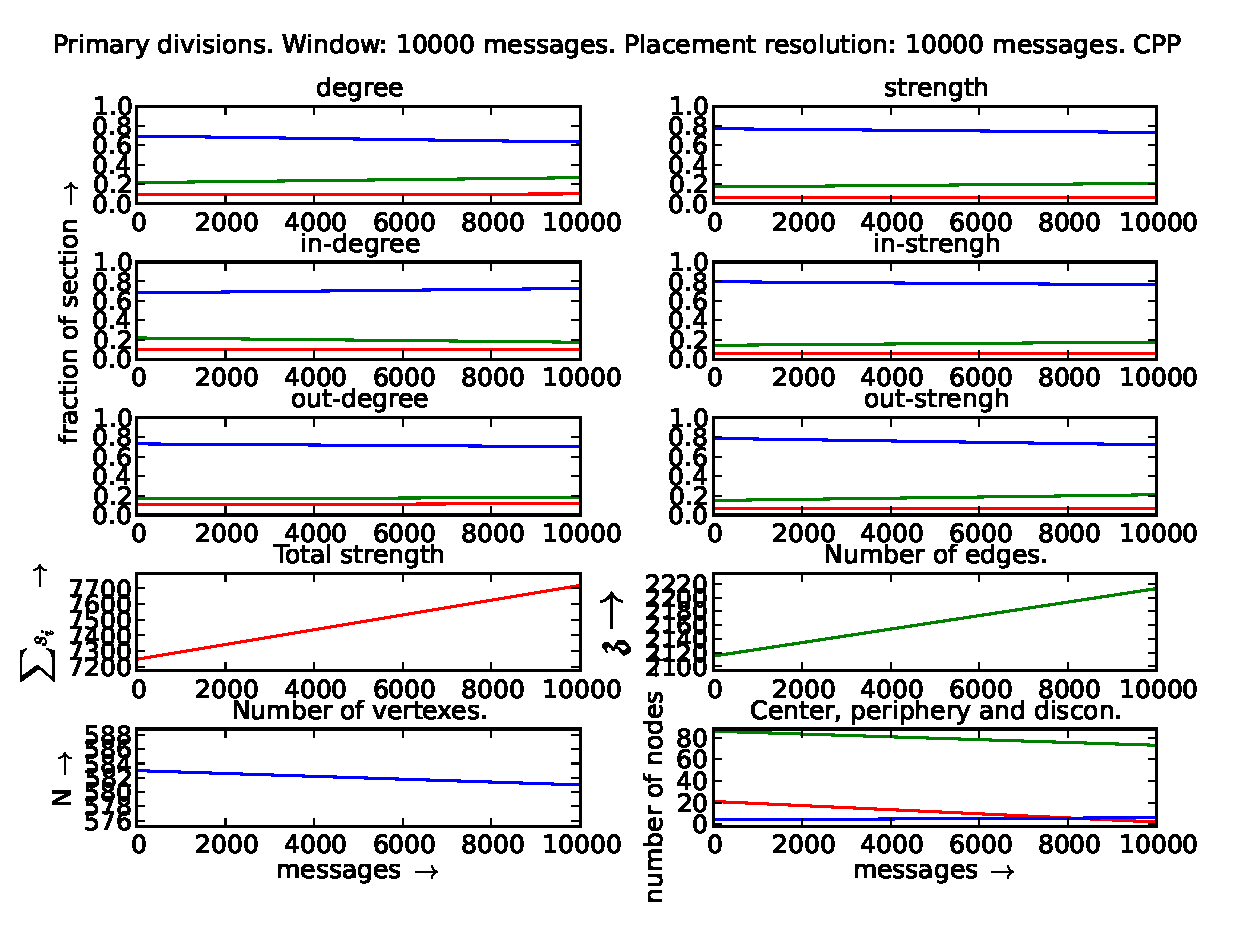
\includegraphics[width=\textwidth]{figs/CPP/10000}
    \caption{Distribution of vertices with respect to each centrality measure: in and out degrees and strengths. CPP Std library official mailing list. In the first six plots, red is fraction of hubs, green is the fraction of intermediary and blue is for peripheral fraction. On the last plot, red is the center (maximum distance to another vertex is equal to radius), blue is periphery (maximum distance equals to diameter) of the giant component. On the same graph, green counts the disconnected vertices.}
    \label{fig:cpp10000}
\end{figure*}


\begin{figure*}[hbtp] 
   \centering
        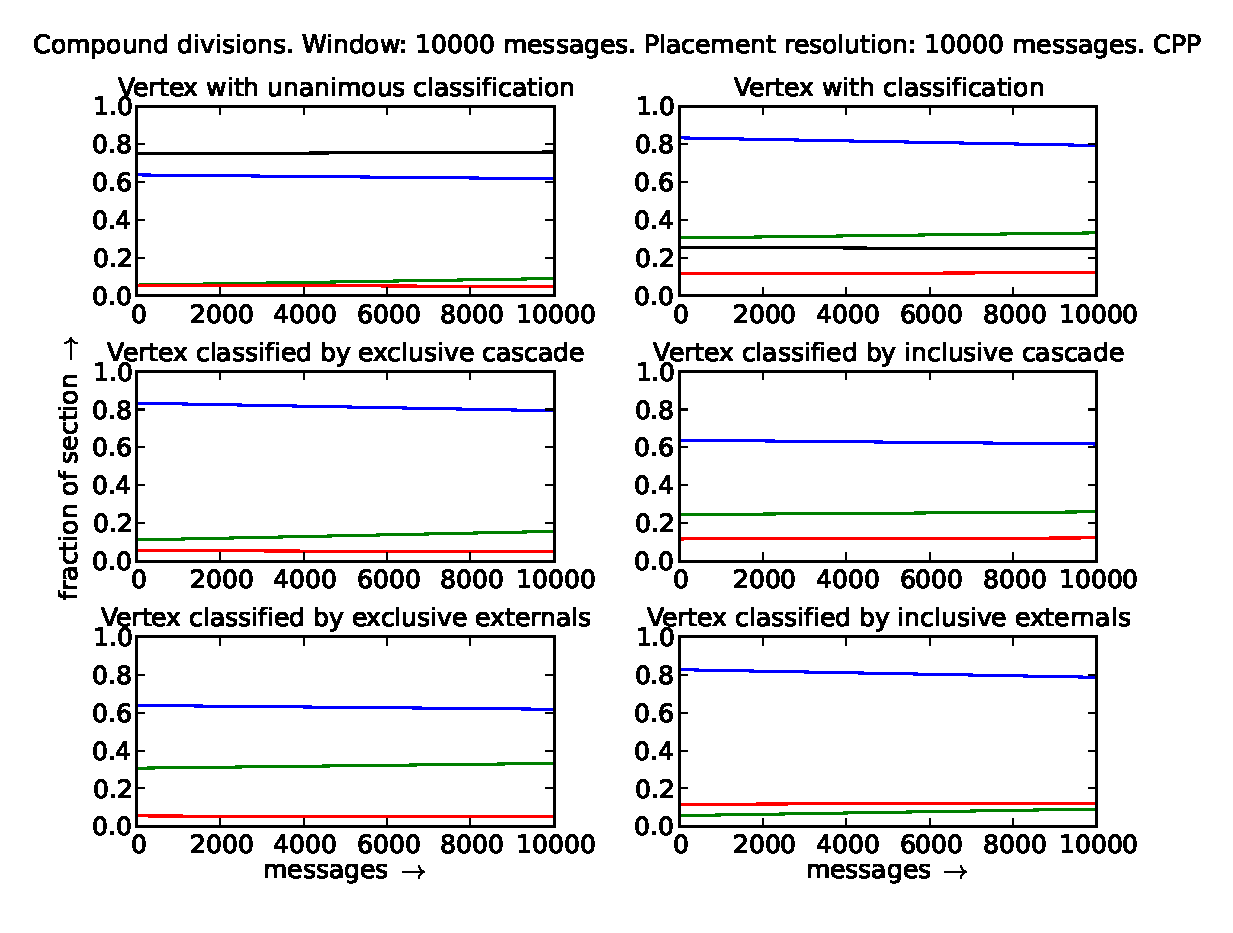
\includegraphics[width=\textwidth]{figs/CPP/10000_2}
    \caption{Distribution of vertex with respect to compound criteria. Red, green and blue designate hubs, intermediary and border (peripheral) vertex fractions. The first two plots exhibit classifications that are not functions. Thus, in the first plot, the fraction of vertices with unique classification is plotted in black. On the second plot, black represents the fraction of vertices that has more than one class: $\frac{\text{number of classifications} - \text{number of nodes}}{\text{number of nodes}}$. Compound criteria is described in Section~\ref{sectioning}.}
    \label{fig:cpp10000_}
\end{figure*}


\begin{figure*}[hbtp] 
   \centering
        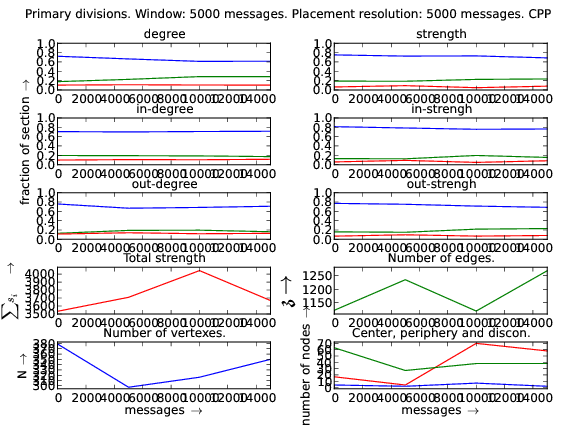
\includegraphics[width=\textwidth]{figs/CPP/5000}
    \caption{Distribution of vertices with respect to each centrality measure: in and out degrees and strengths. CPP Std library official mailing list. In the first six plots, red is fraction of hubs, green is the fraction of intermediary and blue is for peripheral fraction. On the last plot, red is the center (maximum distance to another vertex is equal to radius), blue is periphery (maximum distance equals to diameter) of the giant component. On the same graph, green counts the disconnected vertices.}
    \label{fig:cpp5000}
\end{figure*}


\begin{figure*}[hbtp] 
   \centering
        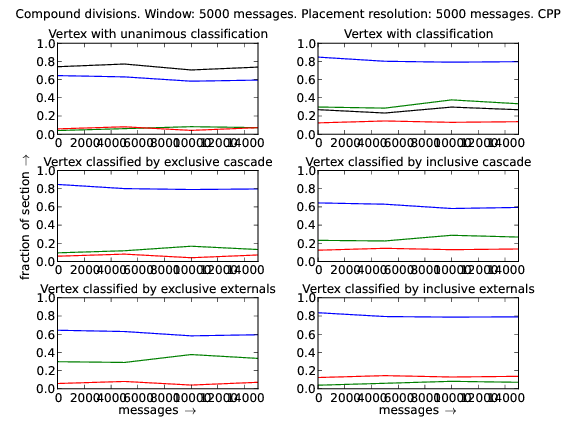
\includegraphics[width=\textwidth]{figs/CPP/5000_2}
    \caption{Distribution of vertex with respect to compound criteria. Red, green and blue designate hubs, intermediary and border (peripheral) vertex fractions. The first two plots exhibit classifications that are not functions. Thus, in the first plot, the fraction of vertices with unique classification in plotted in black. On the second plot, black represents the fraction of vertices that has more than one class: $\frac{\text{number of classifications} - \text{number of nodes}}{\text{number of nodes}}$. Compound criteria is described in Section~\ref{sectioning}.}
    \label{fig:cpp5000_}
\end{figure*}

%%%%
\begin{figure*}[hbtp] 
   \centering
        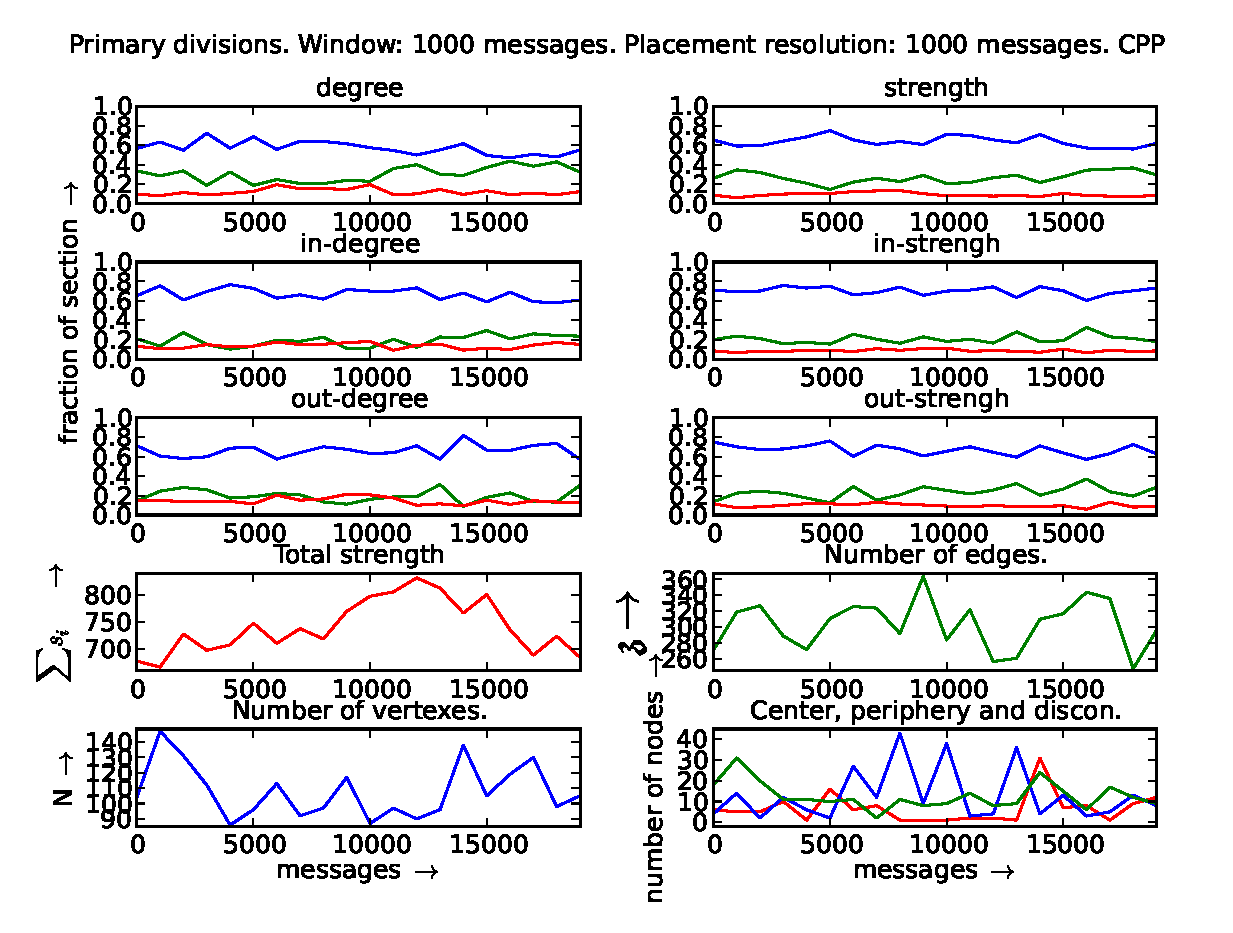
\includegraphics[width=\textwidth]{figs/CPP/1000}
    \caption{Distribution of vertices with respect to each centrality measure: in and out degrees and strengths. CPP Std library official mailing list. In the first six plots, red is fraction of hubs, green is the fraction of intermediary and blue is for peripheral fraction. On the last plot, red is the center (maximum distance to another vertex is equal to radius), blue is periphery (maximum distance equals to diameter) of the giant component. On the same graph, green counts the disconnected vertices.}
    \label{fig:cpp1000}
\end{figure*}


\begin{figure*}[hbtp] 
   \centering
        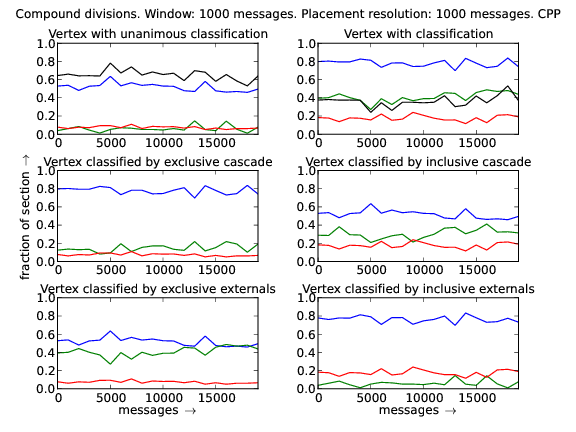
\includegraphics[width=\textwidth]{figs/CPP/1000_2}
    \caption{Distribution of vertex with respect to compound criteria. Red, green and blue designate hubs, intermediary and border (peripheral) vertex fractions. The first two plots exhibit classifications that are not functions. Thus, in the first plot, the fraction of vertices with unique classification in plotted in black. On the second plot, black represents the fraction of vertices that has more than one class: $\frac{\text{number of classifications} - \text{number of nodes}}{\text{number of nodes}}$. Compound criteria is described in Section~\ref{sectioning}.}
    \label{fig:cpp1000_}
\end{figure*}


%%%
\begin{figure*}[hbtp] 
   \centering
        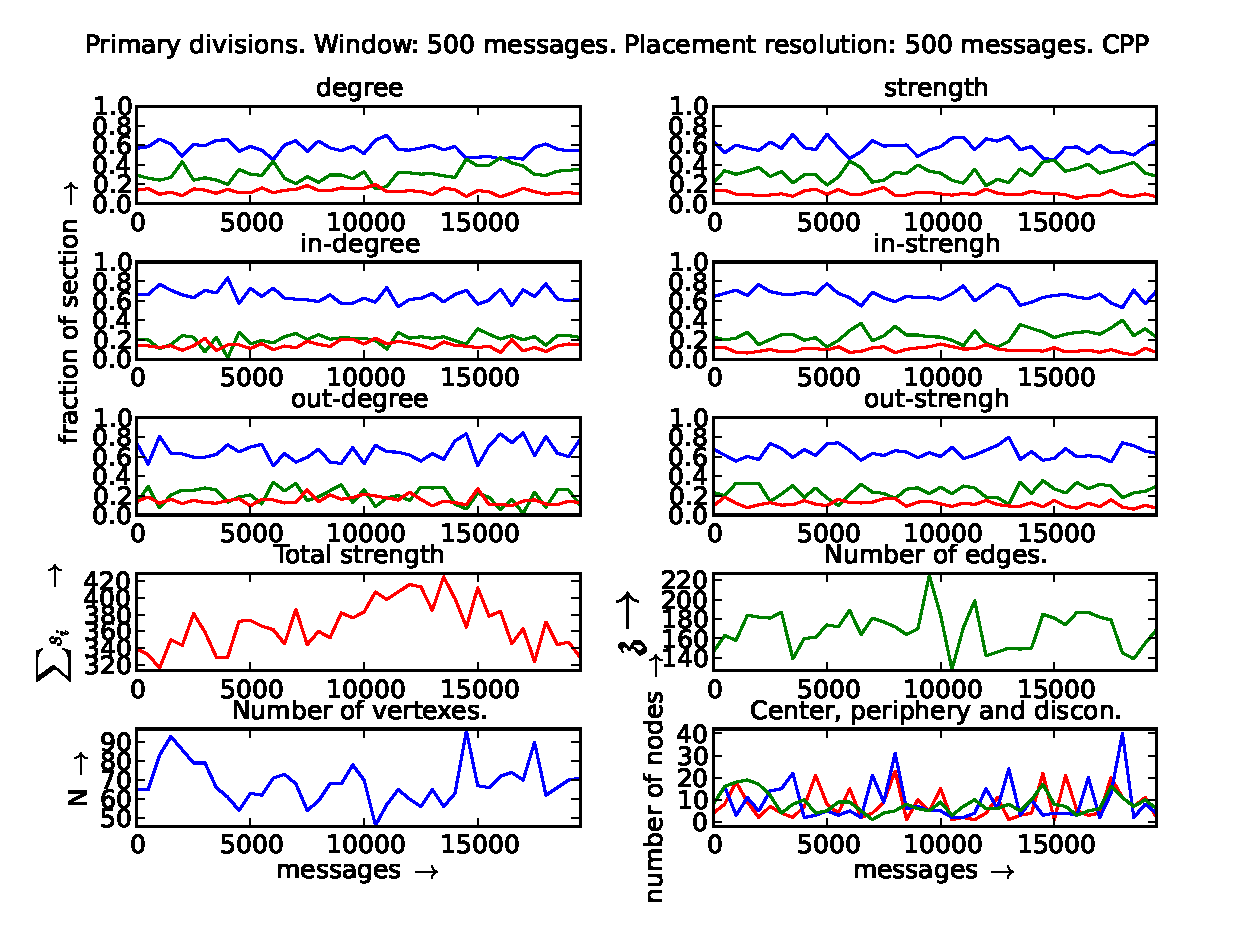
\includegraphics[width=\textwidth]{figs/CPP/500}
    \caption{Distribution of vertices with respect to each centrality measure: in and out degrees and strengths. CPP Std library official mailing list. In the first six plots, red is fraction of hubs, green is the fraction of intermediary and blue is for peripheral fraction. On the last plot, red is the center (maximum distance to another vertex is equal to radius), blue is periphery (maximum distance equals to diameter) of the giant component. On the same graph, green counts the disconnected vertices.}
    \label{fig:cpp500}
\end{figure*}


\begin{figure*}[hbtp] 
   \centering
        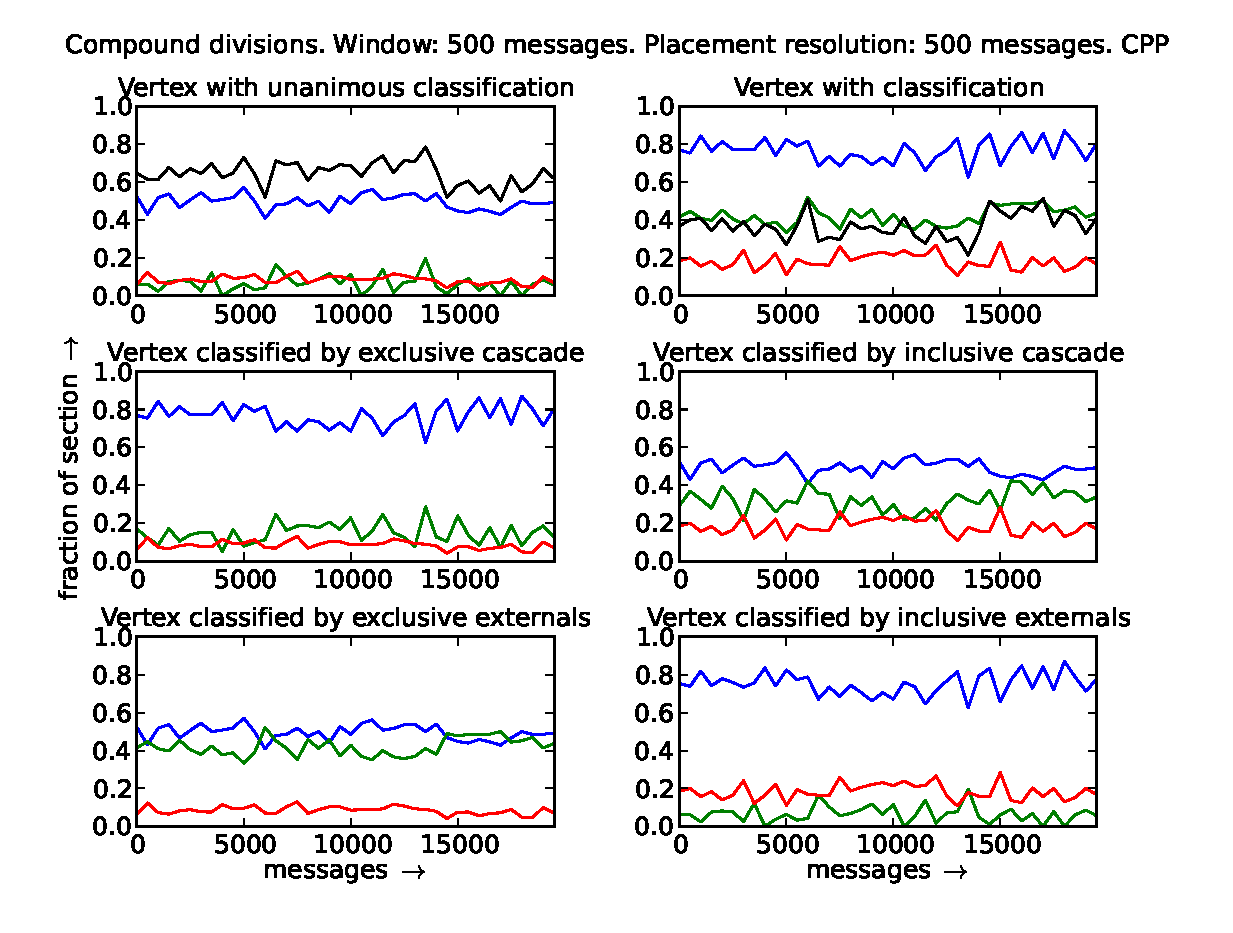
\includegraphics[width=\textwidth]{figs/CPP/500_2}
    \caption{Distribution of vertex with respect to compound criteria. Red, green and blue designate hubs, intermediary and border (peripheral) vertex fractions. The first two plots exhibit classifications that are not functions. Thus, in the first plot, the fraction of vertices with unique classification in plotted in black. On the second plot, black represents the fraction of vertices that has more than one class: $\frac{\text{number of classifications} - \text{number of nodes}}{\text{number of nodes}}$. Compound criteria is described in Section~\ref{sectioning}.}
    \label{fig:cpp500_}
\end{figure*}


%%%%%%%%%
\begin{figure*}[hbtp] 
   \centering
        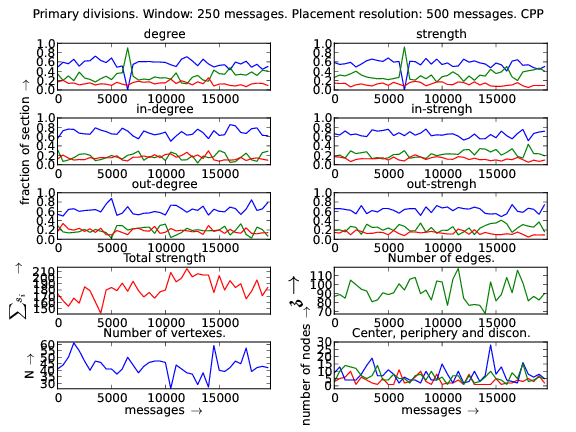
\includegraphics[width=\textwidth]{figs/CPP/250}
    \caption{Distribution of vertices with respect to each centrality measure: in and out degrees and strengths. CPP Std library official mailing list. In the first six plots, red is fraction of hubs, green is the fraction of intermediary and blue is for peripheral fraction. On the last plot, red is the center (maximum distance to another vertex is equal to radius), blue is periphery (maximum distance equals to diameter) of the giant component. On the same graph, green counts the disconnected vertices.}
    \label{fig:cpp250}
\end{figure*}


\begin{figure*}[hbtp] 
   \centering
        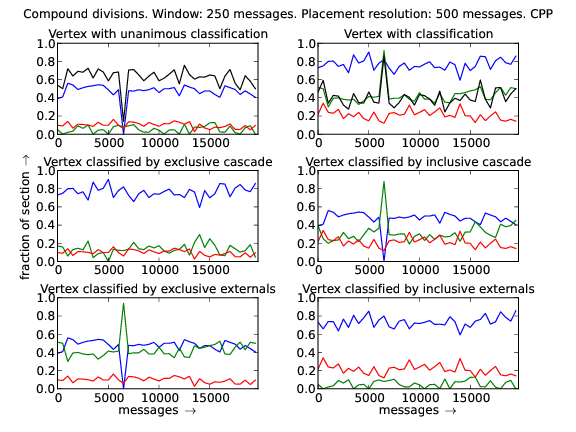
\includegraphics[width=\textwidth]{figs/CPP/250_2}
    \caption{Distribution of vertex with respect to compound criteria. Red, green and blue designate hubs, intermediary and border (peripheral) vertex fractions. The first two plots exhibit classifications that are not functions. Thus, in the first plot, the fraction of vertices with unique classification in plotted in black. On the second plot, black represents the fraction of vertices that has more than one class: $\frac{\text{number of classifications} - \text{number of nodes}}{\text{number of nodes}}$. Compound criteria is described in Section~\ref{sectioning}.}
    \label{fig:cpp250_}
\end{figure*}


%%%%%%%
\begin{figure*}[hbtp] 
   \centering
        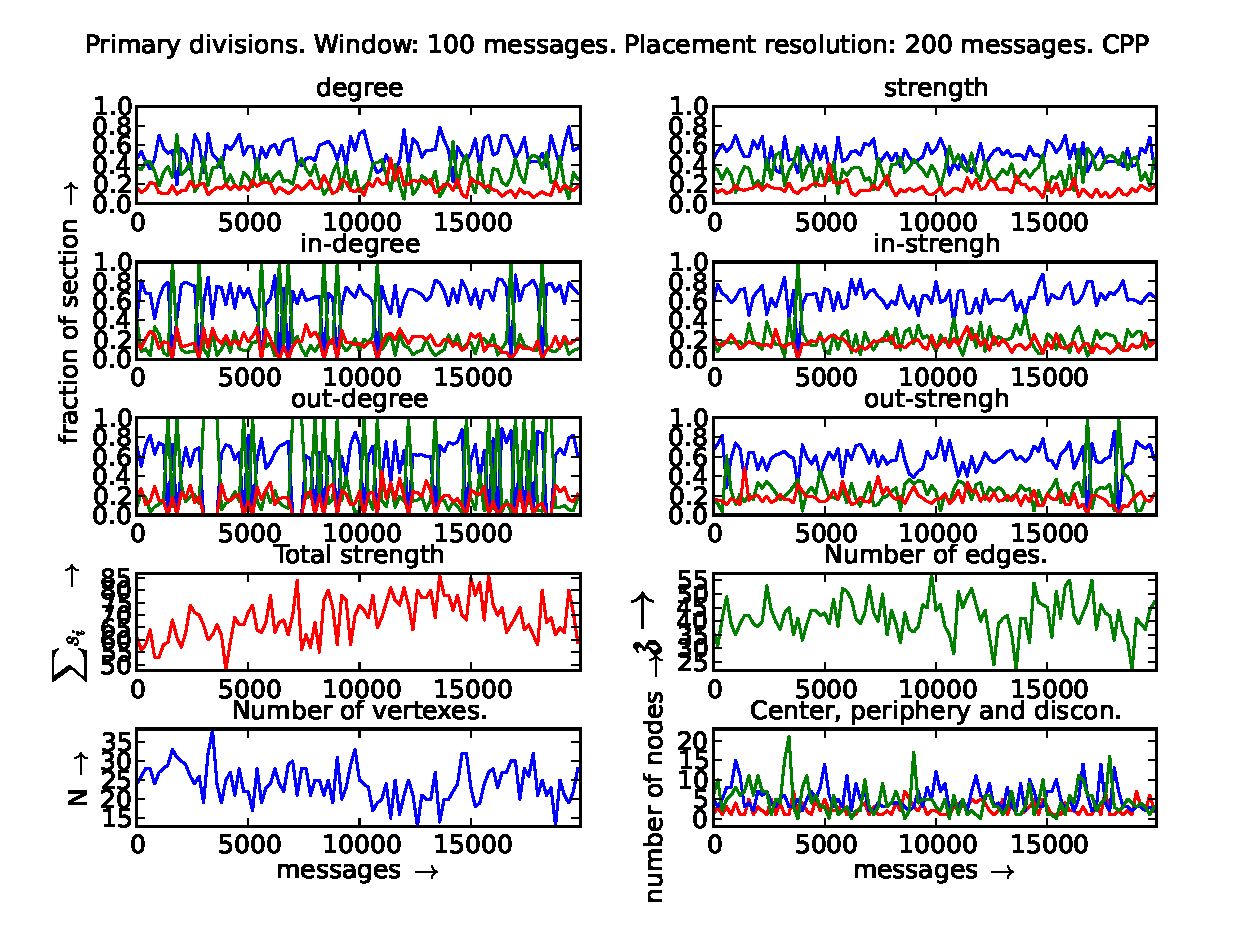
\includegraphics[width=\textwidth]{figs/CPP/100}
    \caption{Distribution of vertices with respect to each centrality measure: in and out degrees and strengths. CPP Std library official mailing list. In the first six plots, red is fraction of hubs, green is the fraction of intermediary and blue is for peripheral fraction. On the last plot, red is the center (maximum distance to another vertex is equal to radius), blue is periphery (maximum distance equals to diameter) of the giant component. On the same graph, green counts the disconnected vertices.}
    \label{fig:cpp100}
\end{figure*}


\begin{figure*}[hbtp] 
   \centering
        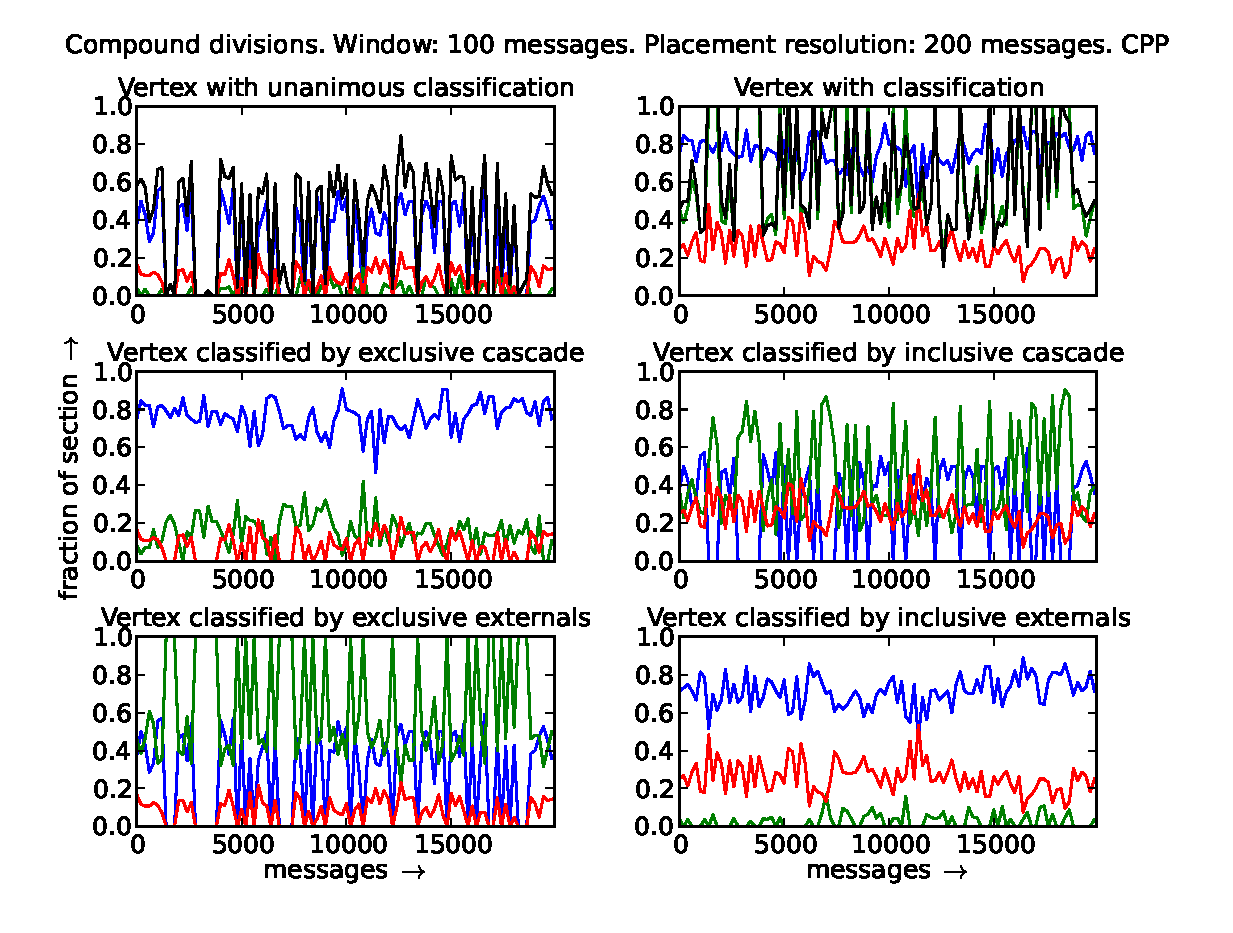
\includegraphics[width=\textwidth]{figs/CPP/100_2}
    \caption{Distribution of vertex with respect to compound criteria. Red, green and blue designate hubs, intermediary and border (peripheral) vertex fractions. The first two plots exhibit classifications that are not functions. Thus, in the first plot, the fraction of vertices with unique classification in plotted in black. On the second plot, black represents the fraction of vertices that has more than one class: $\frac{\text{number of classifications} - \text{number of nodes}}{\text{number of nodes}}$. Compound criteria is described in Section~\ref{sectioning}.}
    \label{fig:cpp100_}
\end{figure*}

%%%%%%%%%%
\begin{figure*}[hbtp] 
   \centering
        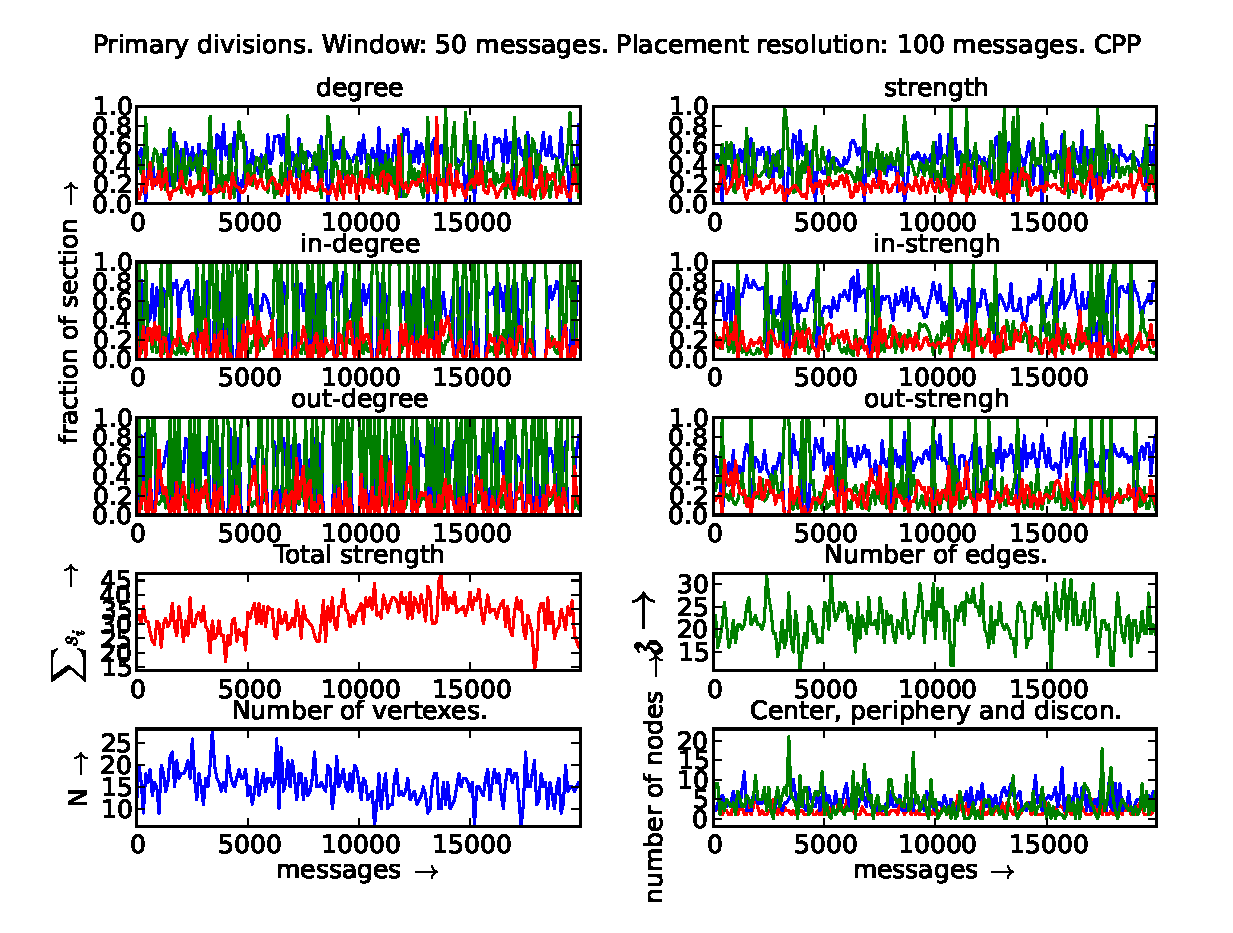
\includegraphics[width=\textwidth]{figs/CPP/50}
    \caption{Distribution of vertices with respect to each centrality measure: in and out degrees and strengths. CPP Std library official mailing list. In the first six plots, red is fraction of hubs, green is the fraction of intermediary and blue is for peripheral fraction. On the last plot, red is the center (maximum distance to another vertex is equal to radius), blue is periphery (maximum distance equals to diameter) of the giant component. On the same graph, green counts the disconnected vertices.}
    \label{fig:cpp50}
\end{figure*}


\begin{figure*}[hbtp] 
   \centering
        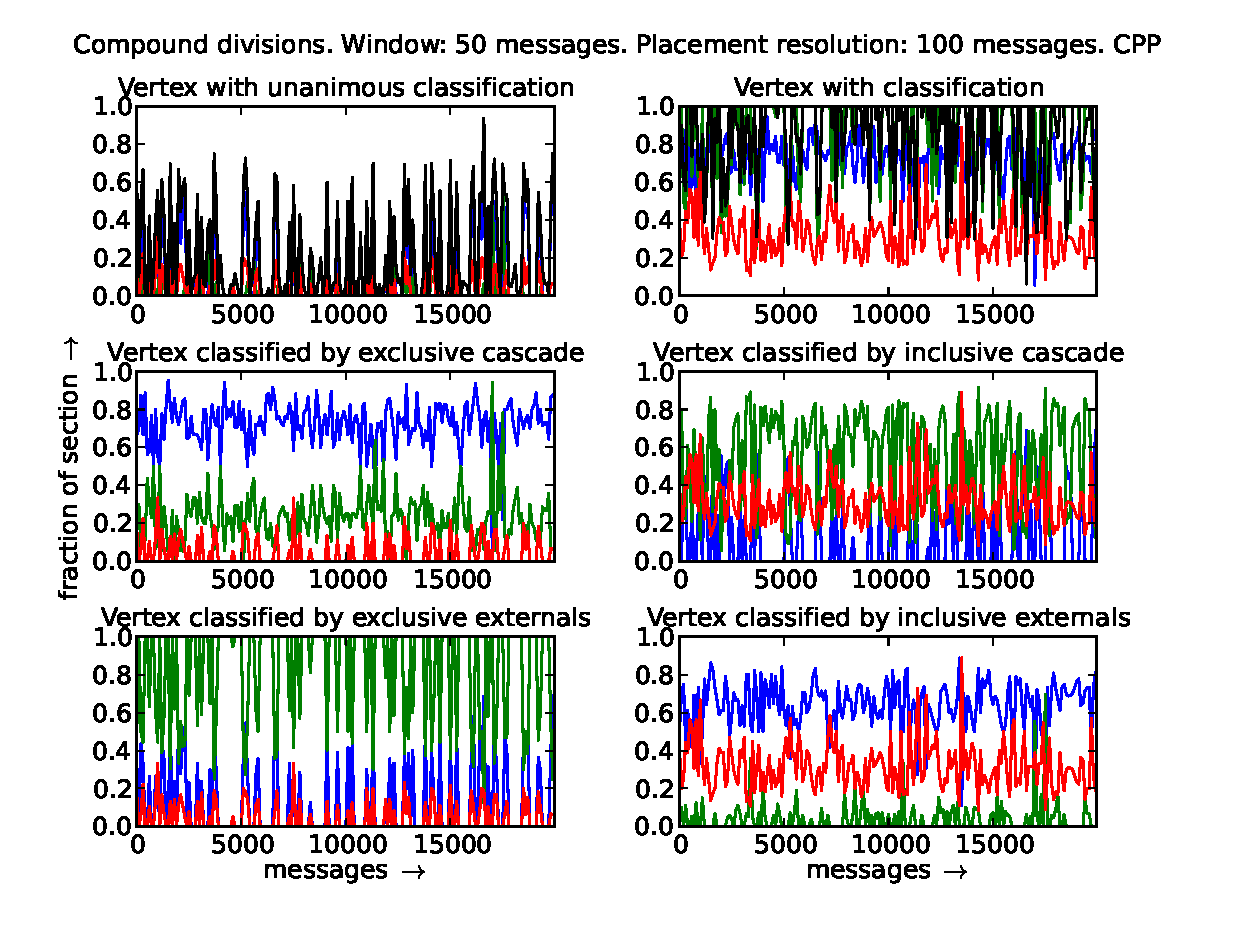
\includegraphics[width=\textwidth]{figs/CPP/50_2}
    \caption{Distribution of vertex with respect to compound criteria. Red, green and blue designate hubs, intermediary and border (peripheral) vertex fractions. The first two plots exhibit classifications that are not functions. Thus, in the first plot, the fraction of vertices with unique classification in plotted in black. On the second plot, black represents the fraction of vertices that has more than one class: $\frac{\text{number of classifications} - \text{number of nodes}}{\text{number of nodes}}$. Compound criteria is described in Section~\ref{sectioning}.}
    \label{fig:cpp50_}
\end{figure*}


\begin{figure*}[hbtp] 
   \centering
        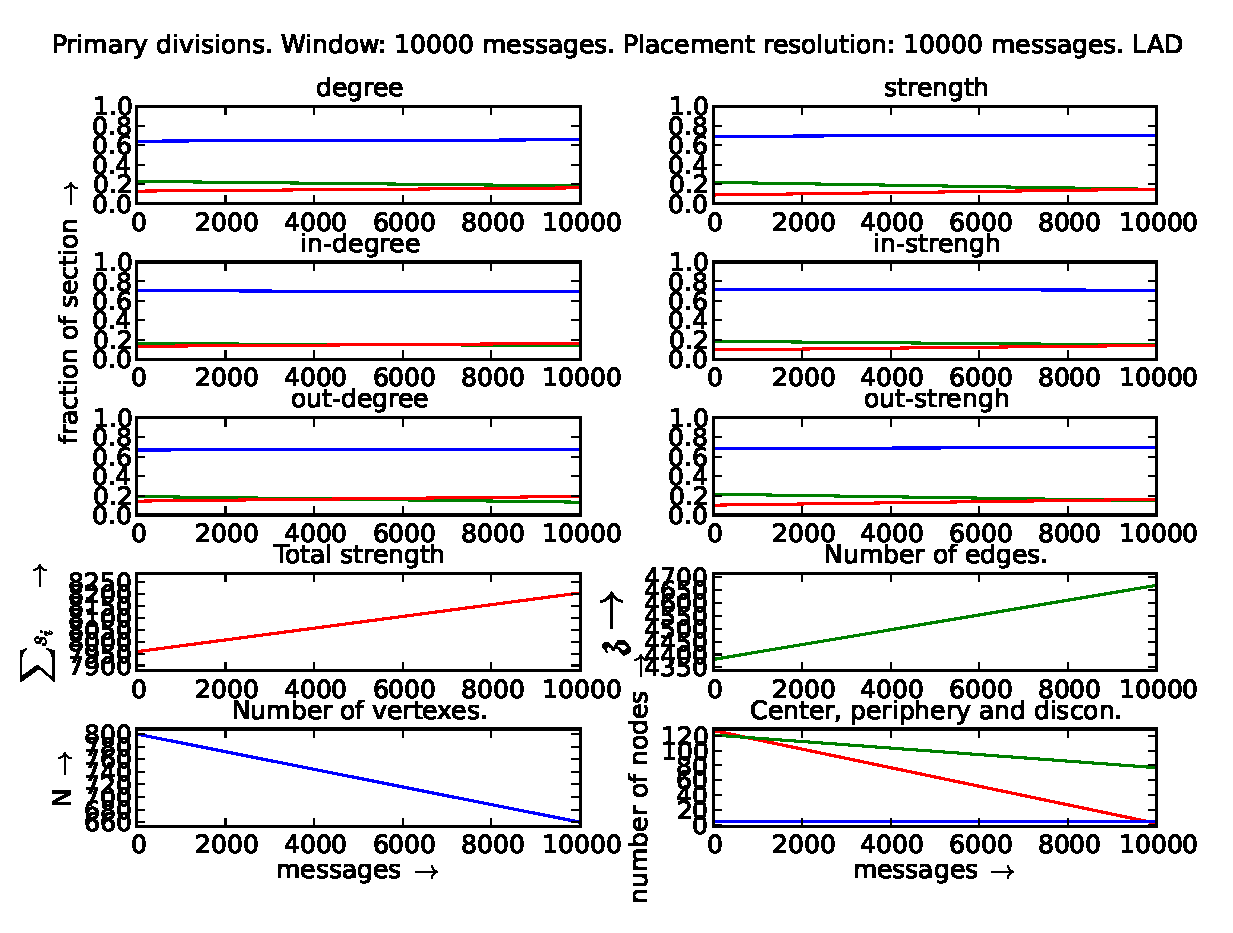
\includegraphics[width=\textwidth]{figs/LAD/10000}
    \caption{Distribution of vertices with respect to each centrality measure: in and out degrees and strengths. Linux Audio Users (LAD) official mailing list. In the first six plots, red is fraction of hubs, green is the fraction of intermediary and blue is for peripheral fraction. On the last plot, red is the center (maximum distance to another vertex is equal to radius), blue is periphery (maximum distance equals to diameter) of the giant component. On the same graph, green counts the disconnected vertices.}
    \label{fig:lad10000}
\end{figure*}


\begin{figure*}[hbtp] 
   \centering
        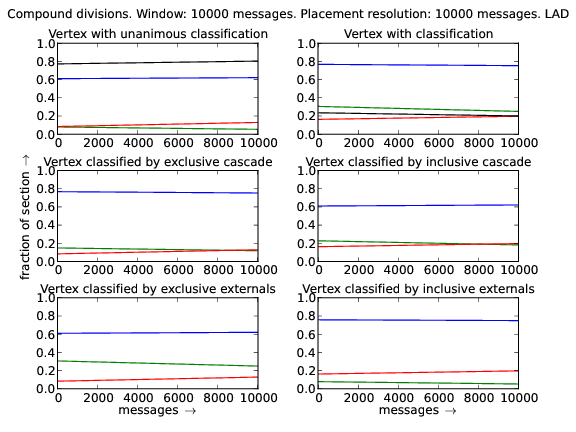
\includegraphics[width=\textwidth]{figs/LAD/10000_2}
    \caption{Distribution of vertex with respect to compound criteria. Red, green and blue designate hubs, intermediary and border (peripheral) vertex fractions. The first two plots exhibit classifications that are not functions. Thus, in the first plot, the fraction of vertices with unique classification in plotted in black. On the second plot, black represents the fraction of vertices that has more than one class: $\frac{\text{number of classifications} - \text{number of nodes}}{\text{number of nodes}}$. Compound criteria is described in Section~\ref{sectioning}.}
    \label{fig:lad10000_}
\end{figure*}


\begin{figure*}[hbtp] 
   \centering
        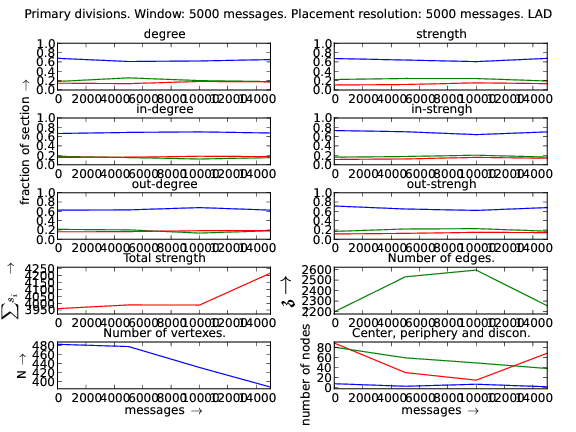
\includegraphics[width=\textwidth]{figs/LAD/5000}
    \caption{Distribution of vertices with respect to each centrality measure: in and out degrees and strengths. Linux Audio Users (LAD) official mailing list. In the first six plots, red is fraction of hubs, green is the fraction of intermediary and blue is for peripheral fraction. On the last plot, red is the center (maximum distance to another vertex is equal to radius), blue is periphery (maximum distance equals to diameter) of the giant component. On the same graph, green counts the disconnected vertices.}
    \label{fig:lad5000}
\end{figure*}


\begin{figure*}[hbtp] 
   \centering
        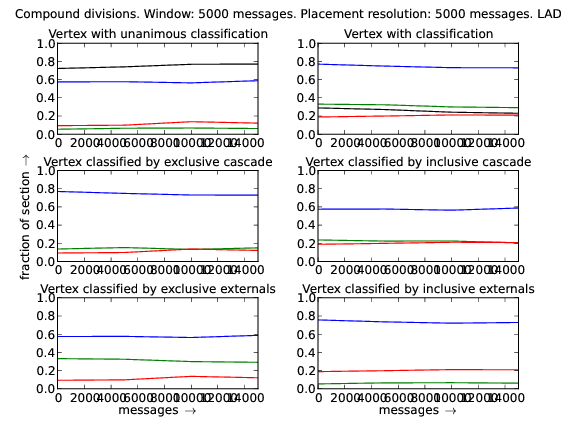
\includegraphics[width=\textwidth]{figs/LAD/5000_2}
    \caption{Distribution of vertex with respect to compound criteria. Red, green and blue designate hubs, intermediary and border (peripheral) vertex fractions. The first two plots exhibit classifications that are not functions. Thus, in the first plot, the fraction of vertices with unique classification in plotted in black. On the second plot, black represents the fraction of vertices that has more than one class: $\frac{\text{number of classifications} - \text{number of nodes}}{\text{number of nodes}}$. Compound criteria is described in Section~\ref{sectioning}.}
    \label{fig:lad5000_}
\end{figure*}

\begin{figure*}[hbtp] 
   \centering
        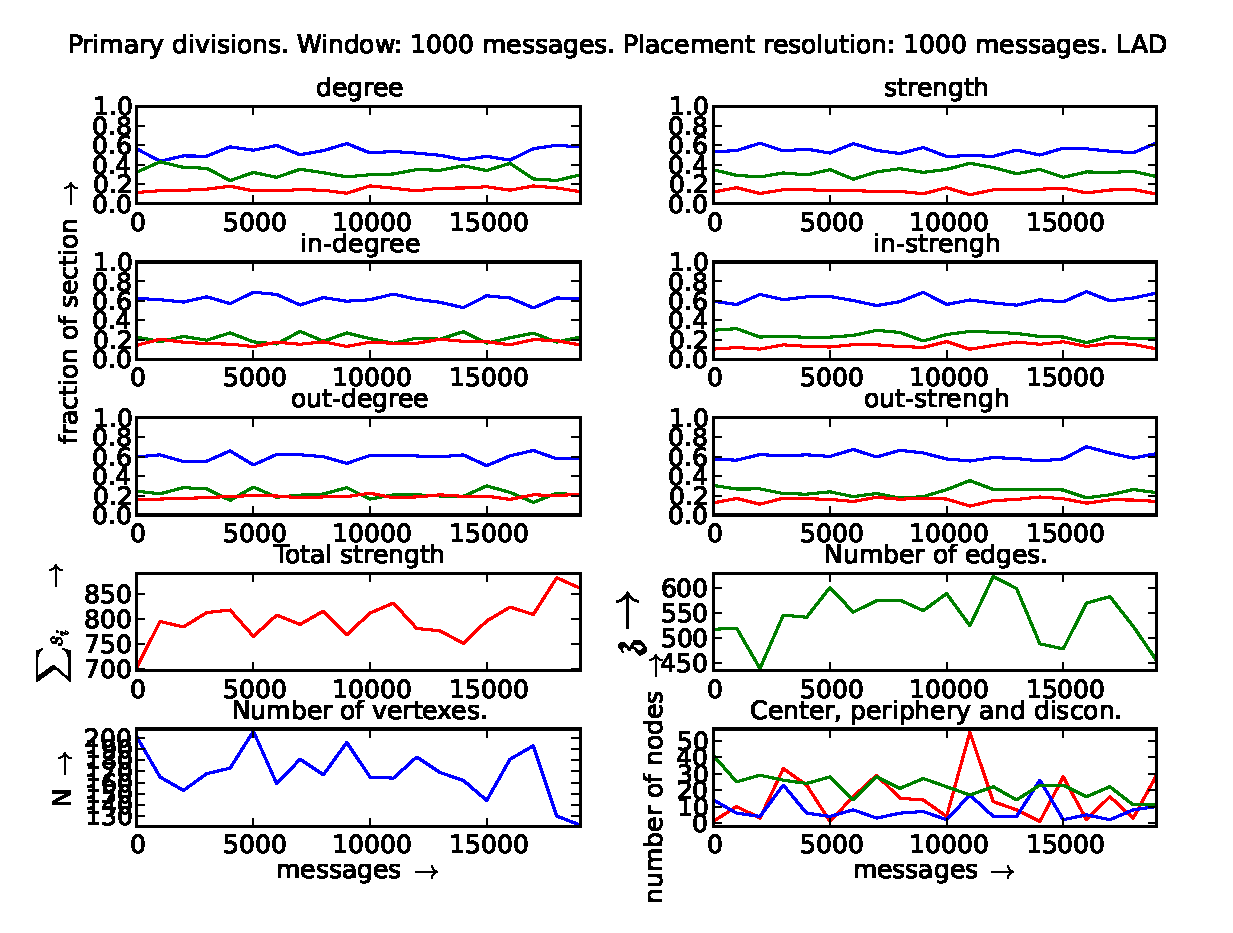
\includegraphics[width=\textwidth]{figs/LAD/1000}
    \caption{Distribution of vertices with respect to each centrality measure: in and out degrees and strengths. Linux Audio Users (LAD) official mailing list. In the first six plots, red is fraction of hubs, green is the fraction of intermediary and blue is for peripheral fraction. On the last plot, red is the center (maximum distance to another vertex is equal to radius), blue is periphery (maximum distance equals to diameter) of the giant component. On the same graph, green counts the disconnected vertices.}
    \label{fig:lad1000}
\end{figure*}


\begin{figure*}[hbtp] 
   \centering
        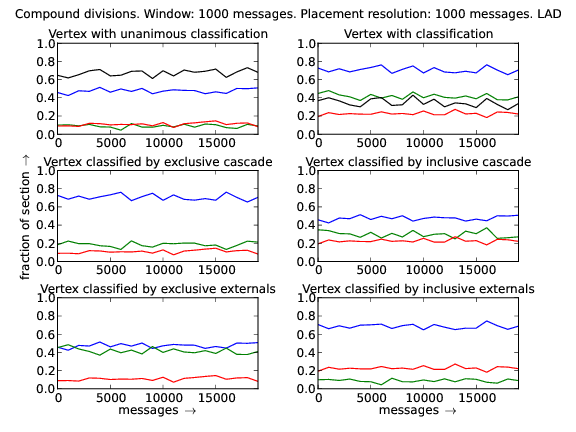
\includegraphics[width=\textwidth]{figs/LAD/1000_2}
    \caption{Distribution of vertex with respect to compound criteria. Red, green and blue designate hubs, intermediary and border (peripheral) vertex fractions. The first two plots exhibit classifications that are not functions. Thus, in the first plot, the fraction of vertices with unique classification in plotted in black. On the second plot, black represents the fraction of vertices that has more than one class: $\frac{\text{number of classifications} - \text{number of nodes}}{\text{number of nodes}}$. Compound criteria is described in Section~\ref{sectioning}.}
    \label{fig:lad1000_}
\end{figure*}


%%%
\begin{figure*}[hbtp] 
   \centering
        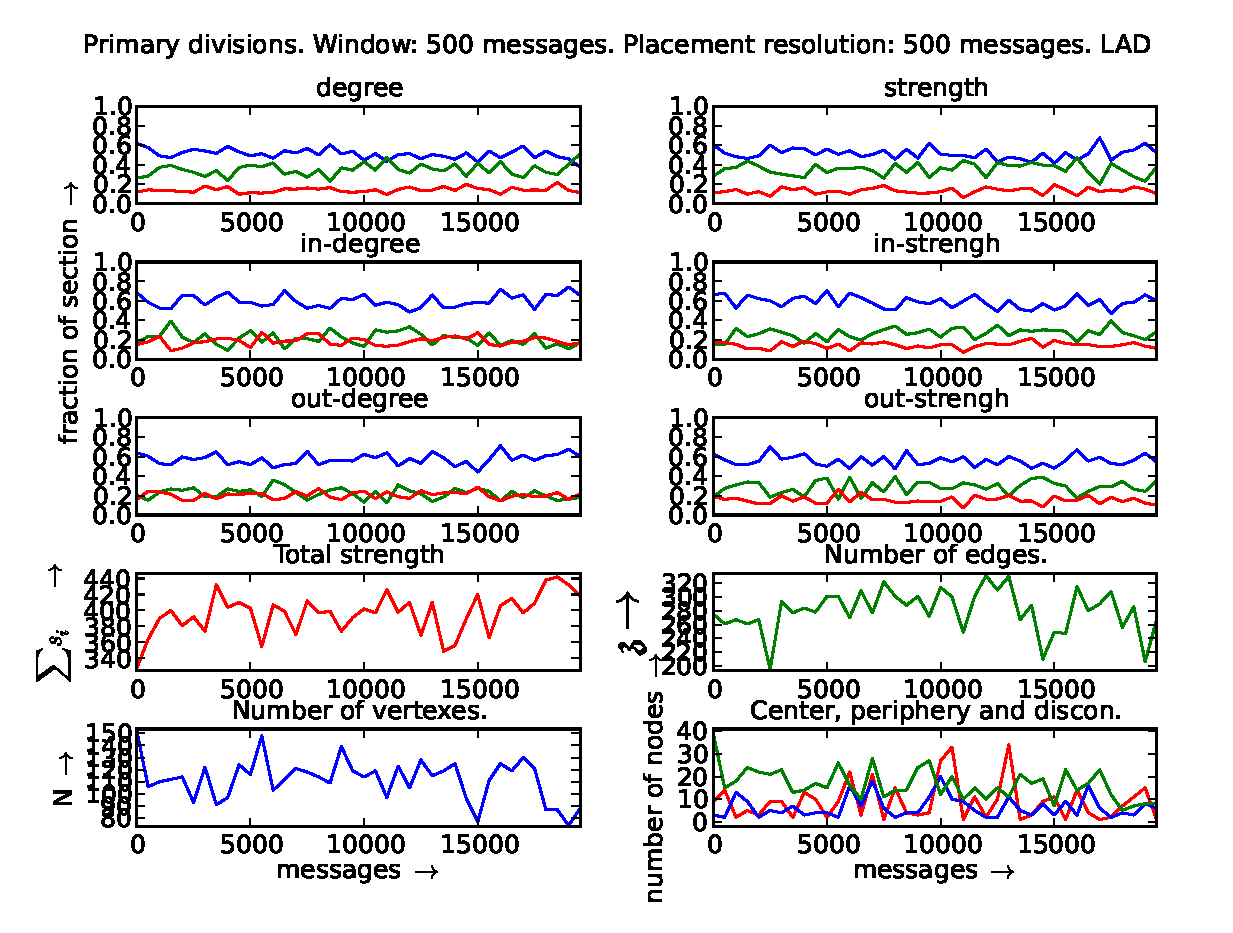
\includegraphics[width=\textwidth]{figs/LAD/500}
    \caption{Distribution of vertices with respect to each centrality measure: in and out degrees and strengths. Linux Audio Users (LAD) official mailing list. In the first six plots, red is fraction of hubs, green is the fraction of intermediary and blue is for peripheral fraction. On the last plot, red is the center (maximum distance to another vertex is equal to radius), blue is periphery (maximum distance equals to diameter) of the giant component. On the same graph, green counts the disconnected vertices.}
    \label{fig:lad500}
\end{figure*}


\begin{figure*}[hbtp] 
   \centering
        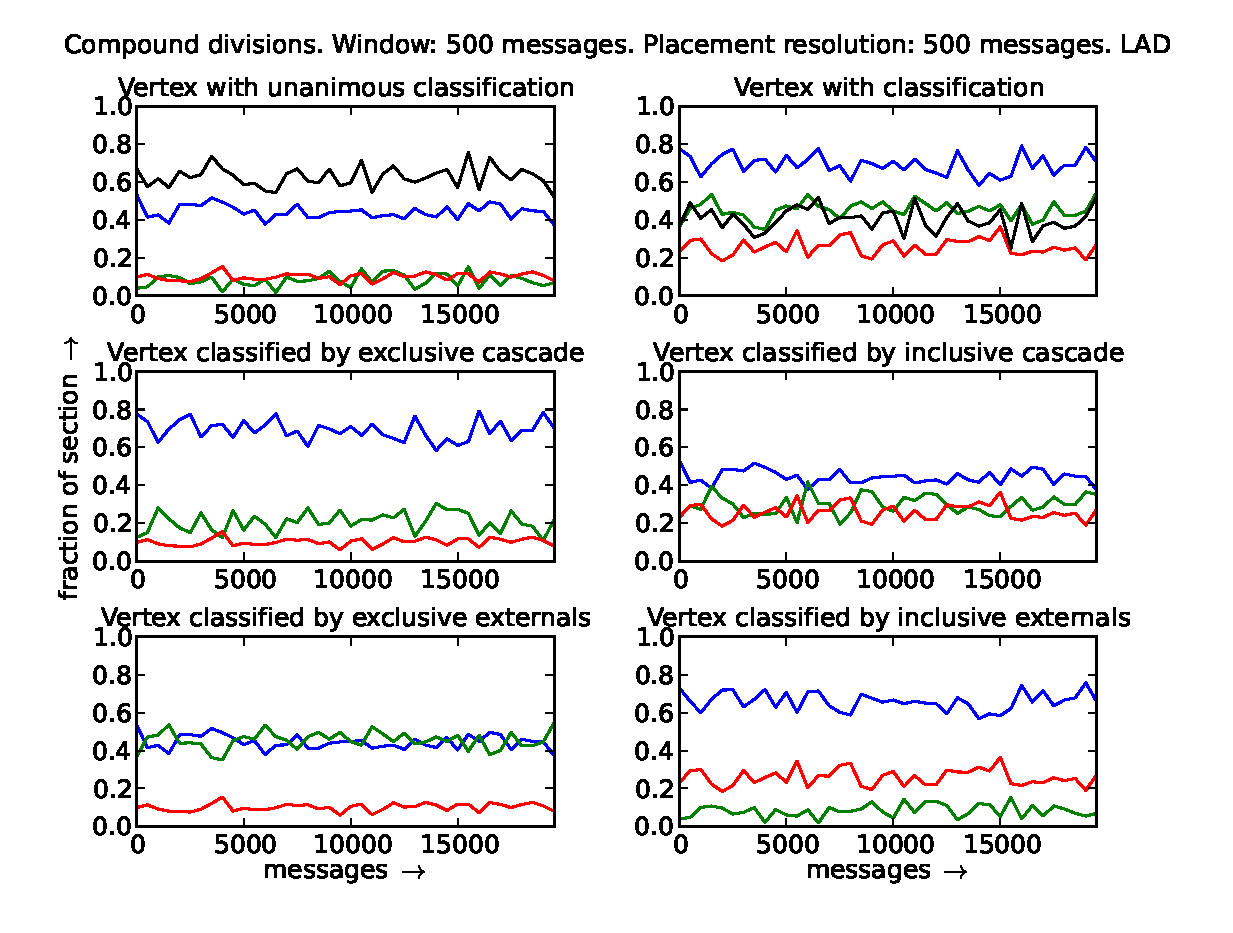
\includegraphics[width=\textwidth]{figs/LAD/500_2}
    \caption{Distribution of vertex with respect to compound criteria. Red, green and blue designate hubs, intermediary and border (peripheral) vertex fractions. The first two plots exhibit classifications that are not functions. Thus, in the first plot, the fraction of vertices with unique classification in plotted in black. On the second plot, black represents the fraction of vertices that has more than one class: $\frac{\text{number of classifications} - \text{number of nodes}}{\text{number of nodes}}$. Compound criteria is described in Section~\ref{sectioning}.}
    \label{fig:lad500_}
\end{figure*}


%%%%%%%%%
\begin{figure*}[hbtp] 
   \centering
        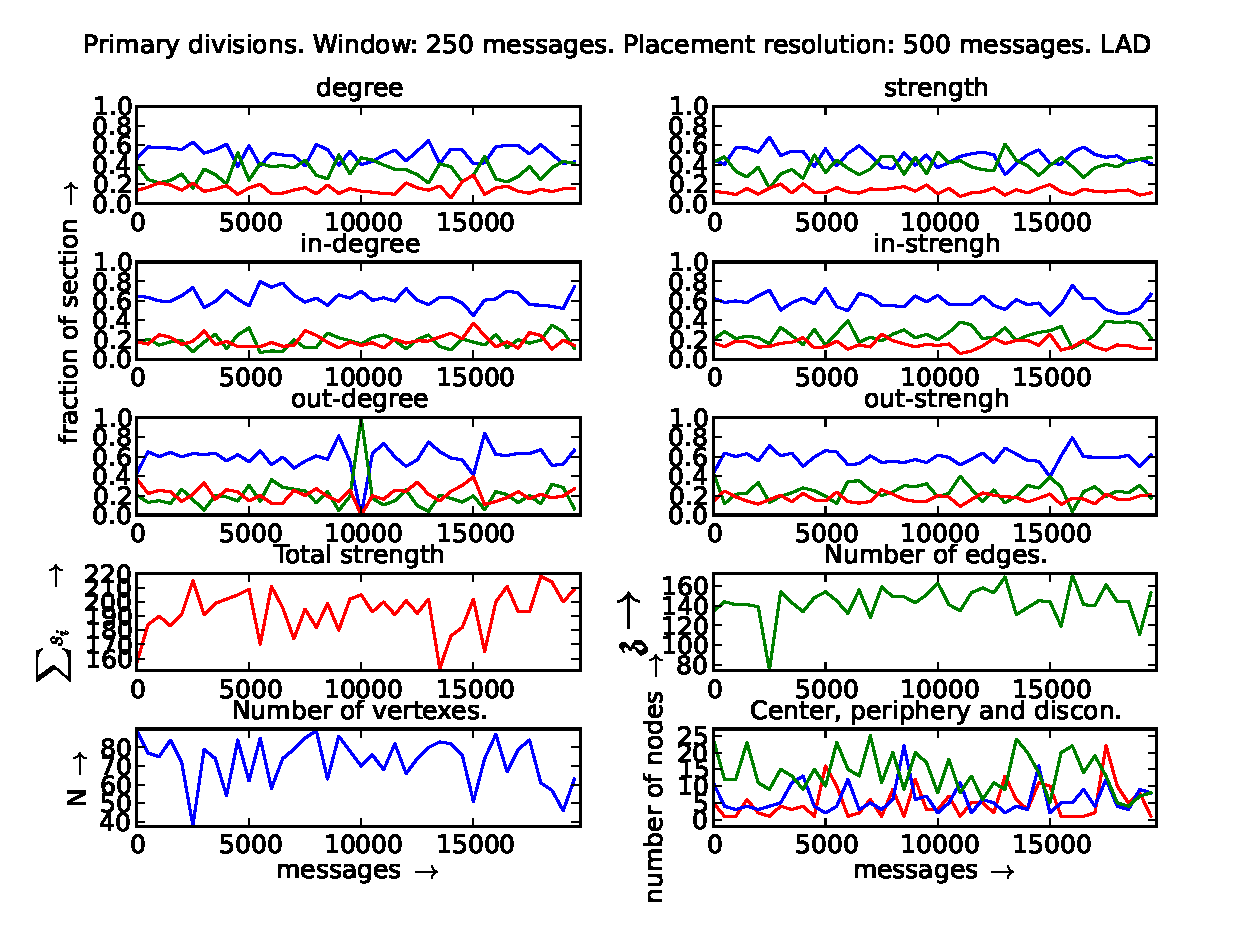
\includegraphics[width=\textwidth]{figs/LAD/250}
    \caption{Distribution of vertices with respect to each centrality measure: in and out degrees and strengths. Linux Audio Users (LAD) official mailing list. In the first six plots, red is fraction of hubs, green is the fraction of intermediary and blue is for peripheral fraction. On the last plot, red is the center (maximum distance to another vertex is equal to radius), blue is periphery (maximum distance equals to diameter) of the giant component. On the same graph, green counts the disconnected vertices.}
    \label{fig:lad250}
\end{figure*}


\begin{figure*}[hbtp] 
   \centering
        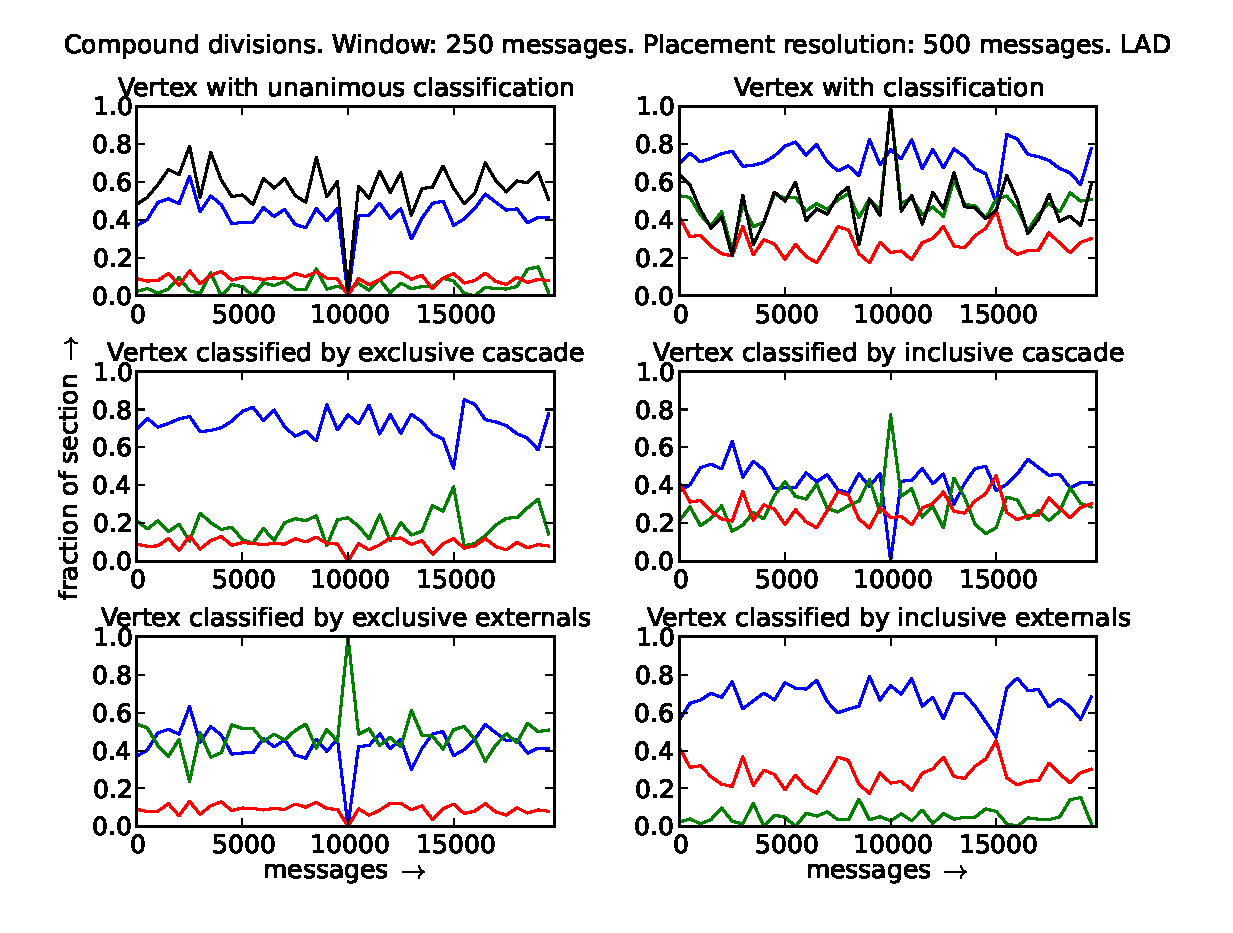
\includegraphics[width=\textwidth]{figs/LAD/250_2}
    \caption{Distribution of vertex with respect to compound criteria. Red, green and blue designate hubs, intermediary and border (peripheral) vertex fractions. The first two plots exhibit classifications that are not functions. Thus, in the first plot, the fraction of vertices with unique classification in plotted in black. On the second plot, black represents the fraction of vertices that has more than one class: $\frac{\text{number of classifications} - \text{number of nodes}}{\text{number of nodes}}$. Compound criteria is described in Section~\ref{sectioning}.}
    \label{fig:lad250_}
\end{figure*}


%%%%%%%
\begin{figure*}[hbtp] 
   \centering
        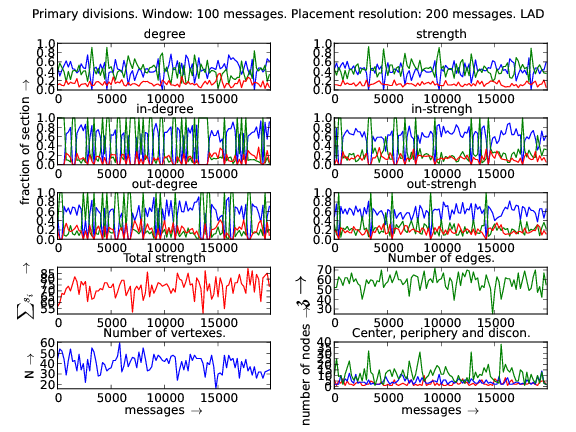
\includegraphics[width=\textwidth]{figs/LAD/100}
    \caption{Distribution of vertices with respect to each centrality measure: in and out degrees and strengths. Linux Audio Users (LAD) official mailing list. In the first six plots, red is fraction of hubs, green is the fraction of intermediary and blue is for peripheral fraction. On the last plot, red is the center (maximum distance to another vertex is equal to radius), blue is periphery (maximum distance equals to diameter) of the giant component. On the same graph, green counts the disconnected vertices.}
    \label{fig:lad100}
\end{figure*}


\begin{figure*}[hbtp] 
   \centering
        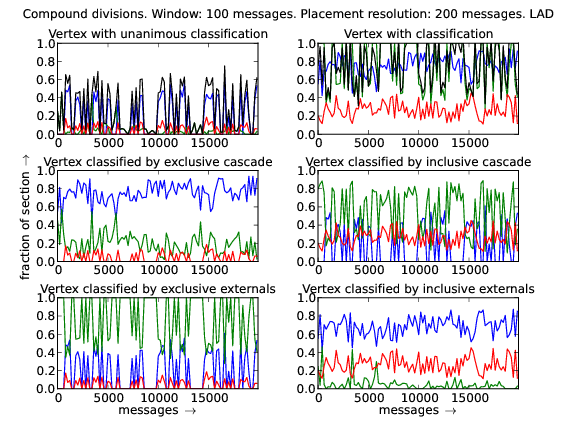
\includegraphics[width=\textwidth]{figs/LAD/100_2}
    \caption{Distribution of vertex with respect to compound criteria. Red, green and blue designate hubs, intermediary and border (peripheral) vertex fractions. The first two plots exhibit classifications that are not functions. Thus, in the first plot, the fraction of vertices with unique classification in plotted in black. On the second plot, black represents the fraction of vertices that has more than one class: $\frac{\text{number of classifications} - \text{number of nodes}}{\text{number of nodes}}$. Compound criteria is described in Section~\ref{sectioning}.}
    \label{fig:lad100_}
\end{figure*}

%%%%%%%%%%
\begin{figure*}[hbtp] 
   \centering
        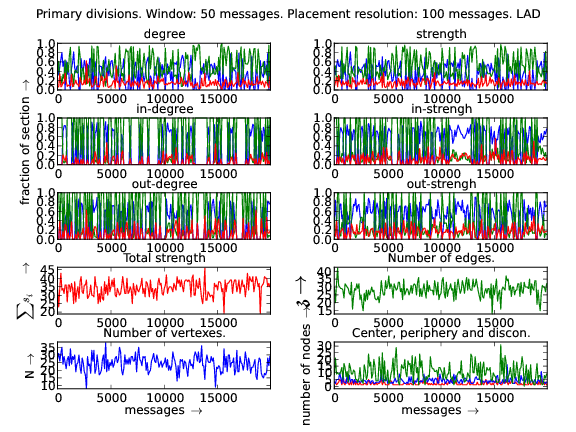
\includegraphics[width=\textwidth]{figs/LAD/50}
    \caption{Distribution of vertices with respect to each centrality measure: in and out degrees and strengths. Linux Audio Users (LAD) official mailing list. In the first six plots, red is fraction of hubs, green is the fraction of intermediary and blue is for peripheral fraction. On the last plot, red is the center (maximum distance to another vertex is equal to radius), blue is periphery (maximum distance equals to diameter) of the giant component. On the same graph, green counts the disconnected vertices.}
    \label{fig:lad50}
\end{figure*}


\begin{figure*}[hbtp] 
   \centering
        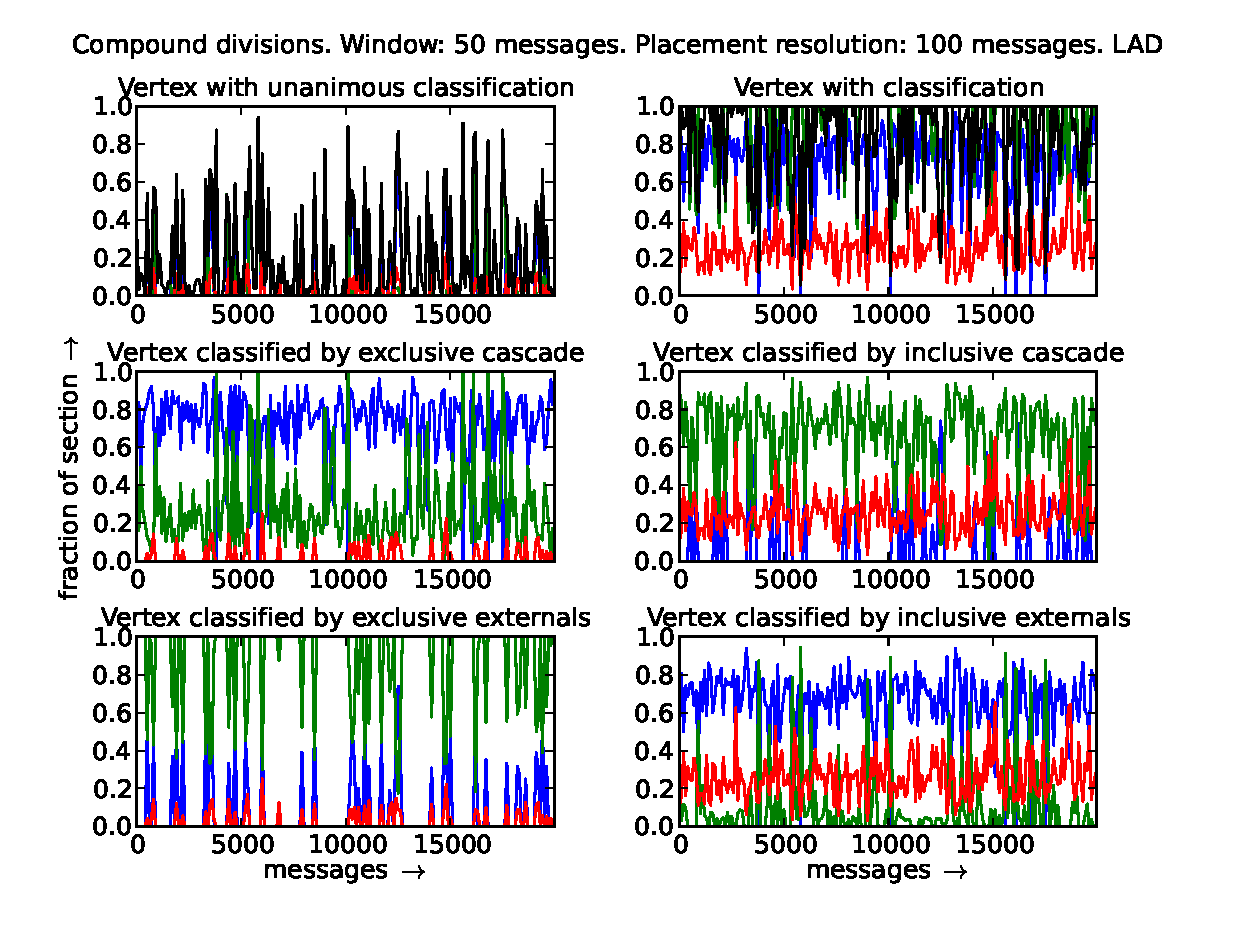
\includegraphics[width=\textwidth]{figs/LAD/50_2}
    \caption{Distribution of vertex with respect to compound criteria. Red, green and blue designate hubs, intermediary and border (peripheral) vertex fractions. The first two plots exhibit classifications that are not functions. Thus, in the first plot, the fraction of vertices with unique classification in plotted in black. On the second plot, black represents the fraction of vertices that has more than one class: $\frac{\text{number of classifications} - \text{number of nodes}}{\text{number of nodes}}$. Compound criteria is described in Section~\ref{sectioning}.}
    \label{fig:lad50_}
\end{figure*}





%
%\begin{figure*}
%    \centering
%        \includegraphics[width=\textwidth]{pcm}
%        \caption{Pulse Code Modulation (PCM) audio: an analogical signal is represented by 25 samples with 4 bits each.}
%        \label{fig:PCM}
%\end{figure*}
%




\nocite{*}
\bibliography{paper}% Produces the bibliography via BibTeX.

\end{document}
%
% ****** End of file aipsamp.tex ******



